\documentclass[11pt,a4paper,oneside]{book}
\usepackage[utf8]{inputenc}
\usepackage[italian]{babel}
\usepackage{amsmath}
\usepackage{amsfonts}
\usepackage{amssymb}
\usepackage[lmargin=3cm,rmargin=3cm,top=4cm,bottom=3cm]{geometry}
\usepackage{graphicx}
\usepackage{url}
\usepackage{listings} %Per inserire codice
\usepackage[usenames]{color} %Per permettere la colorazione dei caratteri
\usepackage[colorlinks=false]{hyperref}
\usepackage{verbatim}
\usepackage{pdfpages}
\addto\captionsitalian{%
\renewcommand{\lstlistingname}{Codice}}
\addto\captionsitalian{%
\renewcommand{\lstlistlistingname}{Elenco dei codici}}


\usepackage{pdfpages}
\author{Giulio Quarenghi}
\title{\large Specifica e diagnosi di sistemi attivi complessi}
\begin{document}

\includepdf[pages={1}]{frontespizio.pdf}
\frontmatter
	\tableofcontents

\chapter*{Ringraziamenti}
Vorrei ringraziare tutte le persone che, direttamente o indirettamente, hanno permesso il raggiungimento di questo traguardo, anche se costituisce per me solo un nuovo punto di partenza, una tappa nel viaggio della vita.\\
Vorrei ringraziare il prof. Lamperti, per la chiarezza, la disponibilità, i preziosi consigli. A lui va la mia riconoscenza e la mia profonda stima.\\
I miei genitori, che mi hanno permesso di ottenere questo risultato, con grandi sacrifici e sostegno incondizionato.\\ 
I miei fratelli, per essere sempre stati per me un esempio da seguire.\\
Martina, per avermi supportato e sopportato in questi ultimi quattro anni e più, per avermi incoraggiato nell'ultimo periodo e per avermi fatto capire ciò che veramente è importante.\\
I miei amici, in particolare Andrea e Boris, e tutti gli altri, per essermi sempre stati vicino.\\
I miei amici e compagni di università, per aver fatto in modo che questi lunghi anni, che solo ora sembrano essere passati così in fretta, non saranno mai dimenticati. 

\begin{flushright}Giulio\end{flushright}

\mainmatter
\chapter{Introduzione}
\chapter{Sistemi a Eventi Discreti}
\chapter{Sistemi Attivi}
In questo capitolo vengono presentate definizioni, modelli ed esempi riguardanti i sistemi attivi tradizionali.
I sistemi attivi rappresentano una classe specifica di sistemi a eventi discreti. Ad un certo livello di astrazione, generalmente, qualsiasi sistema fisico può essere modellato attraverso un comportamento discreto. Un sistema, infatti, non è continuo o discreto di per sé, anche se si può prestare o meno ad una certa scelta nel modello da adottare.
I sistemi attivi sono asincroni; questo significa che gli eventi generati dai componenti sono immagazzinati nei link prima di essere consumati (in maniera asincrona).
Il modello dei sistemi attivi include due tipi fondamentali di elementi: i componenti e i link. Un sistema attivo è una rete di componenti connessi gli uni agli altri per mezzo di link uscenti da terminali di output di alcuni componenti ed entranti nei terminali di input di altri componenti. Il comportamento di ogni componente è descritto da un automa a stati finiti, le cui transizioni tra gli stati sono compiute in base alla consumazione di determinati eventi disponibili nei terminali di input. L'esecuzione di una transizione causa la generazione di eventi trasmessi ai terminali di output del componente. \'E altresì possibile che alcune transizioni non vengano innescate da alcun evento particolare presente nel modello: in questo caso si assume che l'evento scatenante provenga dal mondo esterno al sistema. Il modello comportamentale del componente è assunto essere completo, nel senso che racchiude sia le transizioni normali, sia quelle di guasto.
Un sistema attivo è quindi caratterizzato da una topologia (collegamenti tra componenti) e dal comportamento dei singoli componenti e dei link. Questi ultimi, in un problema generale, potrebbero avere differenti capacità di immagazzinamento (in termini di numero di eventi) e comportamenti diversi nel caso siano colmi (la cosiddetta politica di saturazione).
Il modello globale del sistema è quindi implicitamente dato dalla topologia dell'insieme e dai comportamenti dei singoli componenti e dei link. 

\newpage
\section{Definizioni}
\subsection{Componenti} 
I componenti sono i costituenti base dei sistemi attivi. Ogni componente è caratterizzato da due modelli:
\begin{enumerate}
\item \emph{modello topologico}, secondo il quale un componente è descritto da un insieme di terminali di input, da cui gli eventi in ingresso sono consumati, e da un insieme di terminali di output, dai quali gli eventi in uscita sono generati;
\item \emph{modello comportamentale}, descritto da un automa a stati finiti che ingloba sia il comportamento normale sia le transizioni di guasto, dotato di una funzione di transizione che mappa uno stato e un evento in ingresso in un nuovo stato, generando un sottoinsieme (eventualmente vuoto) di eventi nei terminali di uscita.  
\end{enumerate}

\begin{defn}
Un modello di un componente è un automa:
\begin{center}
	$M_c = (S,E_{in},I,E_{out},O,\tau)$
\end{center}
dove $S$ è l'insieme degli stati, $E_{in}$ è l'insieme degli eventi in ingresso, $I$ è l'insieme dei terminali di input, $E_{out}$ è l'insieme degli eventi in uscita, $O$ è l'insieme dei terminali di output, e $\tau$ è la funzione di transizione (non deterministica):
\begin{center}
	$ \tau : S \times (E_{in} \times I) \times 2^{(E_{out} \times O)} \rightarrow 2^S $.
\end{center}

Un evento è una coppia $(e,\theta)$, dove $e$ è un ingresso (uscita) e $\theta$ un terminale di ingresso (uscita). Un componente particolare può essere visto come una istanza di un modello di componente. 
Una transizione $t$ da uno stato $s$ ad uno stato $s^\prime$ è innescata da un evento in ingresso $(e,x)$ disponibile al terminale di input $x$ e genera l'insieme (possibilmente vuoto) di eventi 
$\{(e_1,y_1), \ldots ,(e_n,y_n)\}$ in corrispondenza dei terminali di output $y_1, \ldots,y_n$, in simboli:
\begin{center}
	$t = s \xrightarrow {(e,x) \Rightarrow (e_1,y_1), \ldots ,(e_n,y_n)} s^{\prime}$.
\end{center}
\end{defn}
\'E implicitamente definito un terminale di input virtuale, chiamato $In$, attraverso il quale giungono gli eventi esterni al sistema.

\begin{ex}\label{ex:modelli}
Si consideri l'esempio di un sistema attivo costituito da un meccanismo di protezione per una linea elettrica. Il componente $p$ rappresenta la protezione (\emph{protection device}), ovvero un sensore che si attiva quando rileva bassa tensione ai capi della linea. Il componente $b$ rappresenta il \emph{breaker}, ovvero il dispositivo che, comandato dalla protezione, si apre isolando la linea elettrica e prevenendo il cortocircuito, oppure si chiude riconnettendo la rete. Nella figure \ref{fig:model_p} e \ref{fig:model_b}  sono rappresentati, rispettivamente, i modelli relativi alla protezione e quelli riferiti al breaker.
Il componente di protezione non possiede terminali di input e ha un terminale di output $o$, mentre il breaker dispone solamente di un terminale di input $i$.
La protezione può essere nello stato inattivo \emph{idle} quando non viene rilevato alcun cortocircuito, oppure nello stato \emph{awaken}, nel momento in cui la tensione si abbassa oltre una certa soglia. Quando viene rilevato un cortocircuito, il componente $p$ può compiere le transizioni $p_1$, che genera un evento $op$ per comandare l'apertura del breaker, o $p_3$, che a causa di un malfunzionamento genera invece un evento $cl$ per comandare la chiusura del breaker. Quando il cortocircuito svanisce, il componente torna nello stato $idle$ percorrendo la transizione $p_2$, che genera l'evento $cl$, oppure tramite $p_4$, che genera in maniera difettosa l'evento $op$.
Il breaker può essere aperto ($open$) o chiuso ($closed$). Quando è chiuso e un evento $op$ è disponibile in corrispondenza del terminale $i$, il breaker $b$ può percorrere la transizione $b_1$ che lo apre o $b_3$ con la quale resta chiuso (guasto). Quando il componente è aperto, le transizioni possibili sono $b_2$ se il breaker si apre, $b_4$ se a causa di un guasto rimane chiuso. Le transizioni $b_5$ e $b_6$ non cambiano lo stato del componente.
Un sunto delle transizioni relative ai due componenti è fornito nelle tabelle \ref{tab:p_trans} e \ref{tab:b_trans}.
\end{ex}

\begin{figure}[htbp]
\centering
\subfigure[topologia protezione]
{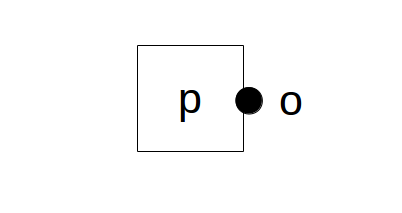
\includegraphics[scale=0.4]{./Img/sa/top_protection.png}}
\hspace{10mm}
\subfigure[comportamento protezione]
{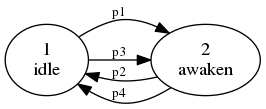
\includegraphics[scale=0.5]{./Img/sa/model_protection.png}}
\caption{Modello del componente $p$}
\label{fig:model_p}
\end{figure}

\begin{figure}[htbp]
\centering
\subfigure[topologia breaker]
{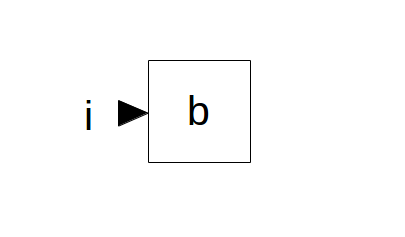
\includegraphics[scale=0.4]{./Img/sa/top_breaker.png}}
\hspace{10mm}
\subfigure[comportamento breaker]
{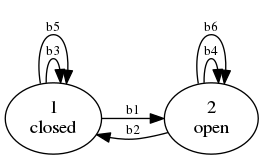
\includegraphics[scale=0.5]{./Img/sa/model_breaker.png}}
\caption{Modello del componente $b$}
\label{fig:model_b}
\end{figure}

\begin{table}[htbp] 
\begin{tabularx}{\textwidth}{l X}
\hline
\textbf{Transizione} & \textbf{Descrizione}\\
\hline\\
$p_1 = idle \xrightarrow{(sh,In) \Rightarrow (op,o)} awaken$ & Rileva un cortocircuito e genera l'evento $op$\\[1mm]
$p_2 = awaken \xrightarrow{(ok,In) \Rightarrow (cl,o)} idle$ & Rileva la fine del cortocircuito e genera l'evento $cl$\\[1mm]
$p_3 = idle \xrightarrow{(sh,In) \Rightarrow (cl,o)} awaken$ & Rileva un cortocircuito ma genera l'evento $cl$\\[1mm]
$p_4 = awaken \xrightarrow{(ok,In) \Rightarrow (op,o)} idle$ & Rileva la fine del cortocircuito ma genera l'evento $op$\\[1mm]
\hline
\end{tabularx}
\caption{Transizioni relative alla protezione}
\label{tab:p_trans}
\end{table}

\begin{table}[htbp] 
\begin{tabularx}{\textwidth}{l X}
\hline
\textbf{Transizione} & \textbf{Descrizione}\\
\hline\\
$b_1 = closed \xrightarrow{(op,i)} open$ & Consuma l'evento $op$ e apre\\[1mm]
$b_2 = open \xrightarrow{(cl,i)} closed$ & Consuma l'evento $cl$ e chiude\\[1mm]
$b_3 = closed \xrightarrow{(op,i)} closed$ & Consuma l'evento $op$ ma rimane chiuso\\[1mm]
$b_4 = open \xrightarrow{(cl,i)} open$ & Consuma l'evento $cl$ ma rimane aperto\\[1mm]
$b_5 = closed \xrightarrow{(cl,i)} closed$ & Consuma l'evento $cl$\\[1mm]
$b_6 = open \xrightarrow{(op,i)} open$ & Consuma l'evento $op$\\[1mm]
\hline
\end{tabularx}
\caption{Transizioni relative al breaker}
\label{tab:b_trans}
\end{table}

\subsection{Link}
Nell'ambito dei sistemi attivi, i componenti sono tra loro connessi per mezzo di link. Ogni link esce da un terminale di output $y$ di un componente $c$ e entra in un terminale di input $x$ di un componente $c^\prime$.
Analogamente a quanto avviene per i componenti, anche i link sono caratterizzati da un modello, che costituisce un'astrazione del link specifico appartenente al sistema.

\begin{defn}
Un modello di un link è una quadrupla
\begin{center}
	$M_l = (x,y,z,w)$
\end{center}
dove $x$ è il terminale di input, $y$ il terminale di output, $z$ la dimensione e $w$ la politica di saturazione.
\end{defn}
Un particolare link $l$ è un'istanza di un modello siffatto, e consiste quindi in un canale di comunicazione unidirezionale fra due componenti distinti $c$ e $c^\prime$, dove un terminale di output $y$ di $c$ e un terminale di input $x$ di $c^\prime$ coincidono rispettivamente con l'input e l'output del link $l$.
La dimensione $z$ rappresenta il numero massimo di eventi che possono essere accodati nel link. 
Indichiamo con $|l|$ la configurazione corrente del link. 
Se il numero di eventi attualmente memorizzati coincide con la dimensione, il link si dice essere saturo.
Quando il link è saturo, la semantica legata al compimento delle transizioni è dettata dalla politica di saturazione $w$, la quale può essere:
\begin{itemize}
\item \emph{lose}: l'evento, non potendo essere memorizzato, viene perso;
\item \emph{override}: l'evento sovrascrive l'ultimo evento nel link;
\item \emph{wait}: la transizione non viene portata a termine fintanto che il link permane nello stato di saturazione, ovvero fino a quando almeno un evento nel link non viene consumato.
\label{saturation}
\end{itemize}
Nell'ambito di questa tesi, si considererà il caso particolare di link di dimensione unitaria e politica di saturazione $wait$ , ovvero $z = 1$ e $w = wait$.
Tale supposizione permette di visualizzare le configurazioni dei link dell'intero sistema come la tupla del contenuto dei terminali di input di ogni componente del sistema. Implicitamente questo significa che ogni evento generato è inserito istantaneamente, se libero, nel terminale (o nei terminali) di input liberi collegati al terminale di output. Se un terminale di destinazione è occupato, la transizione non viene compiuta.

\begin{ex}\label{ex:link}
Con riferimento all'esempio \ref{ex:modelli}, in figura \ref{fig:model_link} è presentato il link $pb$ che collega il terminale di output $o$ della protezione $p$ al terminale di input $i$ del breaker $b$.
\end{ex}

\begin{figure}[htbp]
\centering
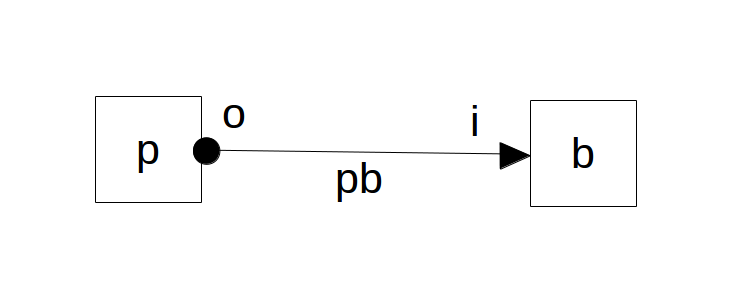
\includegraphics[scale=0.4]{./Img/sa/link.png}
\caption{Modello del sistema attivo $\overline{A}$}
\label{fig:model_link}
\end{figure}

\subsection{Sistema attivo}
Un sistema attivo è una rete di componenti interconnessi per mezzo di link. Ogni componente ed ogni link del sistema sono caratterizzati da un modello e quindi, in generale, più elementi potrebbero avere il medesimo modello. Si assume che più link possano uscire da un terminale di output di un componente, mentre al massimo un link possa entrare in un terminale di input.
Un sistema potrebbe contenere dei terminali che non sono connessi con alcun link: questi vengono chiamati terminali scollegati.

\begin{defn}
Un sistema attivo è una tripla
\begin{center}
	$ A = (C,L,D)$
\end{center}
dove $C$ è l'insieme dei componenti, $L$ l'insieme dei link tra terminali di componenti in $C$, e $D$ è l'insieme dei terminali scollegati. Quest'ultimo insieme può essere visto come l'unione di due insiemi disgiunti:
\begin{center}
	$ D = D_{on} \cup D_{off}$
\end{center}
dove $D_{on}$ è l'insieme dei terminali on scollegati, mentre $D_{off}$ è l'insieme dei terminali off scollegati. 
\end{defn}
Se $D_{on} \neq \emptyset $, il sistema $A$ è detto aperto, altrimenti è detto chiuso. Nel caso $A$ sia chiuso ($D_{on} = \emptyset$), nessun evento è disponibile nei terminali di input di $D_{off}$, mentre gli eventi generati nei terminali di output di $D_{off}$ sono persi.
D'altro canto, se $A$ è aperto, si assume che i terminali scollegati in $D_{on}$ siano connessi attraverso link all'esterno del sistema $A$; quest'ultimo, in altre parole, è come se fosse incorporato in un altro sistema più grande (sconosciuto). Quindi gli eventi generati in terminali di output in $D_{on}$ sono immagazzinati all'interno dei link (sconosciuti) esterni al sistema $A$. Analogamente, il componente in corrispondenza del quale si trova un terminale di input in $D_{on}$ è sensibile a eventi disponibili in quel terminale.

\begin{ex} \label{ex:sa}
Con riferimento agli esempi \ref{ex:modelli} e \ref{ex:link}, il sistema rappresentato in figura \ref{fig:model_link} è un sistema attivo $\overline A = (\{p,b\},\{pb\},\emptyset)$ nel quale non è presente alcun terminale scollegato.
\end{ex}

\subsection{Traiettoria}
Un sistema attivo può essere pensato come una macchina che può essere in uno stato quiescente o in uno stato reattivo. Se si trova nello stato quiescente, i componenti non effettuano alcuna transizione, dal momento che nessun evento è disponibile nei terminali di ingresso. In corrispondenza del verificarsi di un determinato evento, sia esso proveniente dal mondo esterno, sia da un terminale di input scollegato appartenente a $D_{on}$, il sistema evolve nella sua fase reattiva. Dato che il comportamento del sistema è asincrono (non dipende dal tempo), la reazione, detta \emph{traiettoria} (o \emph{storia}), consiste in una sequenza di transizioni compiute da componenti presenti nel sistema.
Ogni transizione di un componente porta il sistema in un nuovo stato, dove uno stato è identificato dallo stato corrente di ogni componente e dallo stato attuali di ogni link. In altre parole, uno stato del sistema attivo è una coppia $(S,Q)$, dove $S$ è la n-pla degli stati dei componenti, mentre $Q$ è la m-pla delle configurazioni dei link, ovvero la m-pla del contenuto dei terminali di input di tutti i componenti.
In questo lavoro di tesi, il focus è sulla cosiddetta diagnosi a posteriori, che avviene quando il sistema ha percorso una traiettoria partendo da uno stato quiescente e tornando in uno stato di quiete, nel quale cioè tutti i terminali di input dei componenti sono vuoti. In questo contesto, una traiettoria completa può essere vista come una sequenza di transizioni che, partendo dallo stato iniziale (quiescente), termina in uno stato finale (anch'esso quiescente).
Una transizione del sistema può essere scritta come:
\begin{center}
	$T = (S,Q) \xrightarrow {t(c)} (S^\prime,Q^\prime)$,
\end{center}
dove $t(c)$ identifica univocamente la transizione $t$ appartenente al modello del componente $c$.
Assumendo che $a_0 = (S_0,Q_0)$ sia lo stato iniziale del sistema, la traiettoria ottenuta partendo da $a_0$ è la sequenza di stati del sistema determinata dall'occorrenza di transizioni $t_1, \ldots , t_k$ attuabili da parte dei singoli componenti:
\begin{center}
$h = a_0 \xrightarrow{t_1(c_1)} a1 \xrightarrow{t_2(c_2)} a2 \ldots \xrightarrow{t_k(c_k)} a_k$.
\end{center}
Ogni stato (non iniziale) dipende quindi dallo stato precedente e dalla particolare transizione che lo porta allo stato corrente, ovvero la coppia $(a_{i-1},t_i(c_i))$. Assumendo che si parta dallo stato iniziale $a_0$ questo ci permette di identificare una traiettoria per mezzo delle sole transizioni dei componenti:
\begin{center}
$h = [t_1(c_1),t_2(c_2), \ldots , t_k(c_k)]$.
\end{center}

\begin{ex} \label{ex:traiettoria}
Con riferimento al sistema attivo in figura \ref{fig:model_link}, si assuma che lo stato iniziale sia la composto dalla tripla $(idle,closed,\epsilon)$ indicante rispettivamente gli stati dei componenti $p$ e $b$ (figure \ref{fig:model_p} e \ref{fig:model_b}) e il contenuto inizialmente vuoto del link $pb$, ovvero del terminale di input $i$ del breaker. Una possibile traiettoria è la seguente:
\begin{center}
$\overline h = (idle,closed,\epsilon) \xrightarrow{p_1(p)} (awaken,closed,op) \xrightarrow{b_1(b)}(awaken,open,\epsilon) \xrightarrow{p_2(p)} (idle,open,cl) \xrightarrow{b_2(b)} (idle,closed,\epsilon)$
\end{center}
che corrisponde alla seguente dinamica:
\begin{enumerate}
\item la protezione rileva un cortocircuito e comanda l'apertura del breaker;
\item il breaker si apre;
\item la protezione rileva la fine del cortocircuito e comanda la chiusura del breaker;
\item il breaker di chiude.
\end{enumerate}
Si noti come lo stato finale della traiettoria $\overline{h}$ coincida con lo stato iniziale della medesima traiettoria. Questa ciclicità permette di inferire la presenza di infinite traiettorie per il sistema attivo in esame, in quanto percorrere un ciclo un diverso numero di volte porta alla percorrenza di traiettorie diverse.
Da osservare, inoltre, come una siffatta dinamica sia esente da guasti: nelle sezioni successive verranno analizzati casi più generali, contraddistinti da malfunzionamenti, e saranno fornite le informazioni necessarie al fine di discriminare le transizioni normali da quelle di guasto.
\end{ex}

\subsection{Behavior Space}
Dato un sistema attivo ed il suo stato iniziale, possono esservi molte traiettorie percorribili, persino infinite. Analogamente a quanto avviene per il comportamento del singolo componente, che può essere descritto nel suo modello come un automa a stati finiti, anche per quanto riguarda le traiettorie dell'intero sistema si può seguire un procedimento analogo. Un automa a stati finiti rappresenta infatti, attraverso un numero di stati e di transizioni finiti, un numero di traiettorie che può essere infinito. Questo è dovuto alla possibile presenza di ciclicità all'interno dell'automa. Tale automa è chiamato \emph{behavior space} e ha come alfabeto l'intero insieme delle transizioni dei singoli componenti del sistema.
Il linguaggio del \emph{behavior space} $Bsp(A)$ con stato iniziale $a_0$ coincide con l'insieme di tutte le possibili traiettorie del sistema $A$ partendo dallo stato $a_0$. 
\begin{defn}
Sia $A = (L,C,D)$ un sistema attivo, dove $C$ è l'insieme di $n$ componenti, mentre $L$ è l'insieme di $m$ link. Il behavior space di $A$ è il DFA
\begin{center}
	$Bsp(A) = (\Sigma,\alpha,\tau,a_0,\alpha_f)$
\end{center}
dove:
\begin{enumerate}
\item $\Sigma$ è l'alfabeto, dato dall'unione delle transizioni dei componenti in $C$;
\item $\alpha$  è l'insieme degli stati $(S,Q)$, con $S = (s_1,\ldots,s_n)$ una n-pla di stati dei componenti in $C$, e $Q = (q_1, \ldots,q_m)$ una m-pla del contenuto dei terminali di input di tutti i componenti;
\item $a_0 = (S_0,Q_0)$ è lo stato iniziale;
\item $\alpha_f$ è l'insieme degli stati finali, ovvero stati in cui $Q = (\epsilon \ldots \epsilon)$;
\item $\tau$ è la funzione di transizione deterministica, $\tau: \alpha \times \Sigma \rightarrow \alpha$, tale che $(S,Q) \xrightarrow{t(c)} (S^\prime, Q^\prime) \in \tau$, dove $S = (s_1, \ldots,s_n)$, $Q = (q_1, \ldots,q_m)$, $S^\prime = (s^\prime_1, \ldots,s^\prime_n)$, $Q^\prime = (q^\prime_1, \ldots,q^\prime_m)$ e
\begin{center}
$t(c) = s \xrightarrow{(e,x) | \{(e_1,y_1), \ldots, (e_p,y_p)\}} s^\prime$
\end{center}
se e solo se:
\begin{itemize}
\item $x = In$, cioè l'evento è disponibile sul terminale di input virtuale sensibile agli eventi esterni al sistema, oppure $x \in D_{on}$, o $e$ è pronto al terminale $x$ all'interno di un link del sistema;
\item Per ogni $i \in [1 \ldots n]$, abbiamo
\begin{center}
$s^\prime_i = \begin{cases} s^\prime & \mbox{se }c_i = c\\ s_i & \mbox{altrimenti} \end{cases}$
\end{center}
cioè per ogni transizione del \emph{behavior space} cambia lo stato relativo al singolo componente coinvolto nella transizione;
\item $Q^\prime$ differisce da $Q$ per le seguenti condizioni:
\begin{itemize}
\item $Q(x) = e \rightarrow Q^\prime(x) = \epsilon$, cioè l'evento in input è consumato;
\item $\forall(e_j,y_j), j \in [1 \ldots p], Q(y_j) = \epsilon \rightarrow Q^\prime(y_j) = e_j$, cioè gli eventi di uscita sono inseriti nei terminali di input connessi ai terminali di output coinvolti nella transizione. 
\end{itemize}
\end{itemize}
\end{enumerate}
\end{defn}
Il \emph{behavior space}, contenendo tutte le possibili traiettorie del sistema, assume dimensioni considerevoli anche con la presenza di pochi componenti e relativi terminali di input. Questo perché la sua dimensione ha una complessità esponenziale nel numero di componenti e link, dato che uno stato del \emph{behavior space} è caratterizzato, nel caso peggiore, da tutte le possibili combinazioni di stati dei componenti e contenuto dei link \footnote{Si tratta di un limite di complessità superiore. In base alle particolari transizioni coinvolte, infatti, non tutte le combinazione sono possibili stati del \emph{behavior space}.}. Per questo motivo, si assume che un automa siffatto non possa essere generato perché troppo costoso, in termini di tempo di esecuzione ma soprattutto di memoria. Nella risoluzione del problema di diagnosi, infatti, verrà generato un automa più contenuto, chiamato semplicemente \emph{behavior}.

\begin{ex}
Il \emph{behavior space} del sistema attivo $\overline{A}$ dell'esempio \ref{ex:sa} è riportato in figura \ref{fig:bsp}. Si considera come stato iniziale $a_0$ lo stato nel quale la protezione è inattiva, il breaker è chiuso e il link $pb$ è vuoto. Gli archi evidenziati rappresentano la particolare traiettoria $\overline{h}$ introdotta nell'esempio \ref{ex:traiettoria}, mentre i nodi con un doppio contorno rappresentano gli stati finali $\alpha_f$ nei quali l'unico link $pb$ del sistema è vuoto.
\end{ex}

\begin{figure}[htbp]
\centering
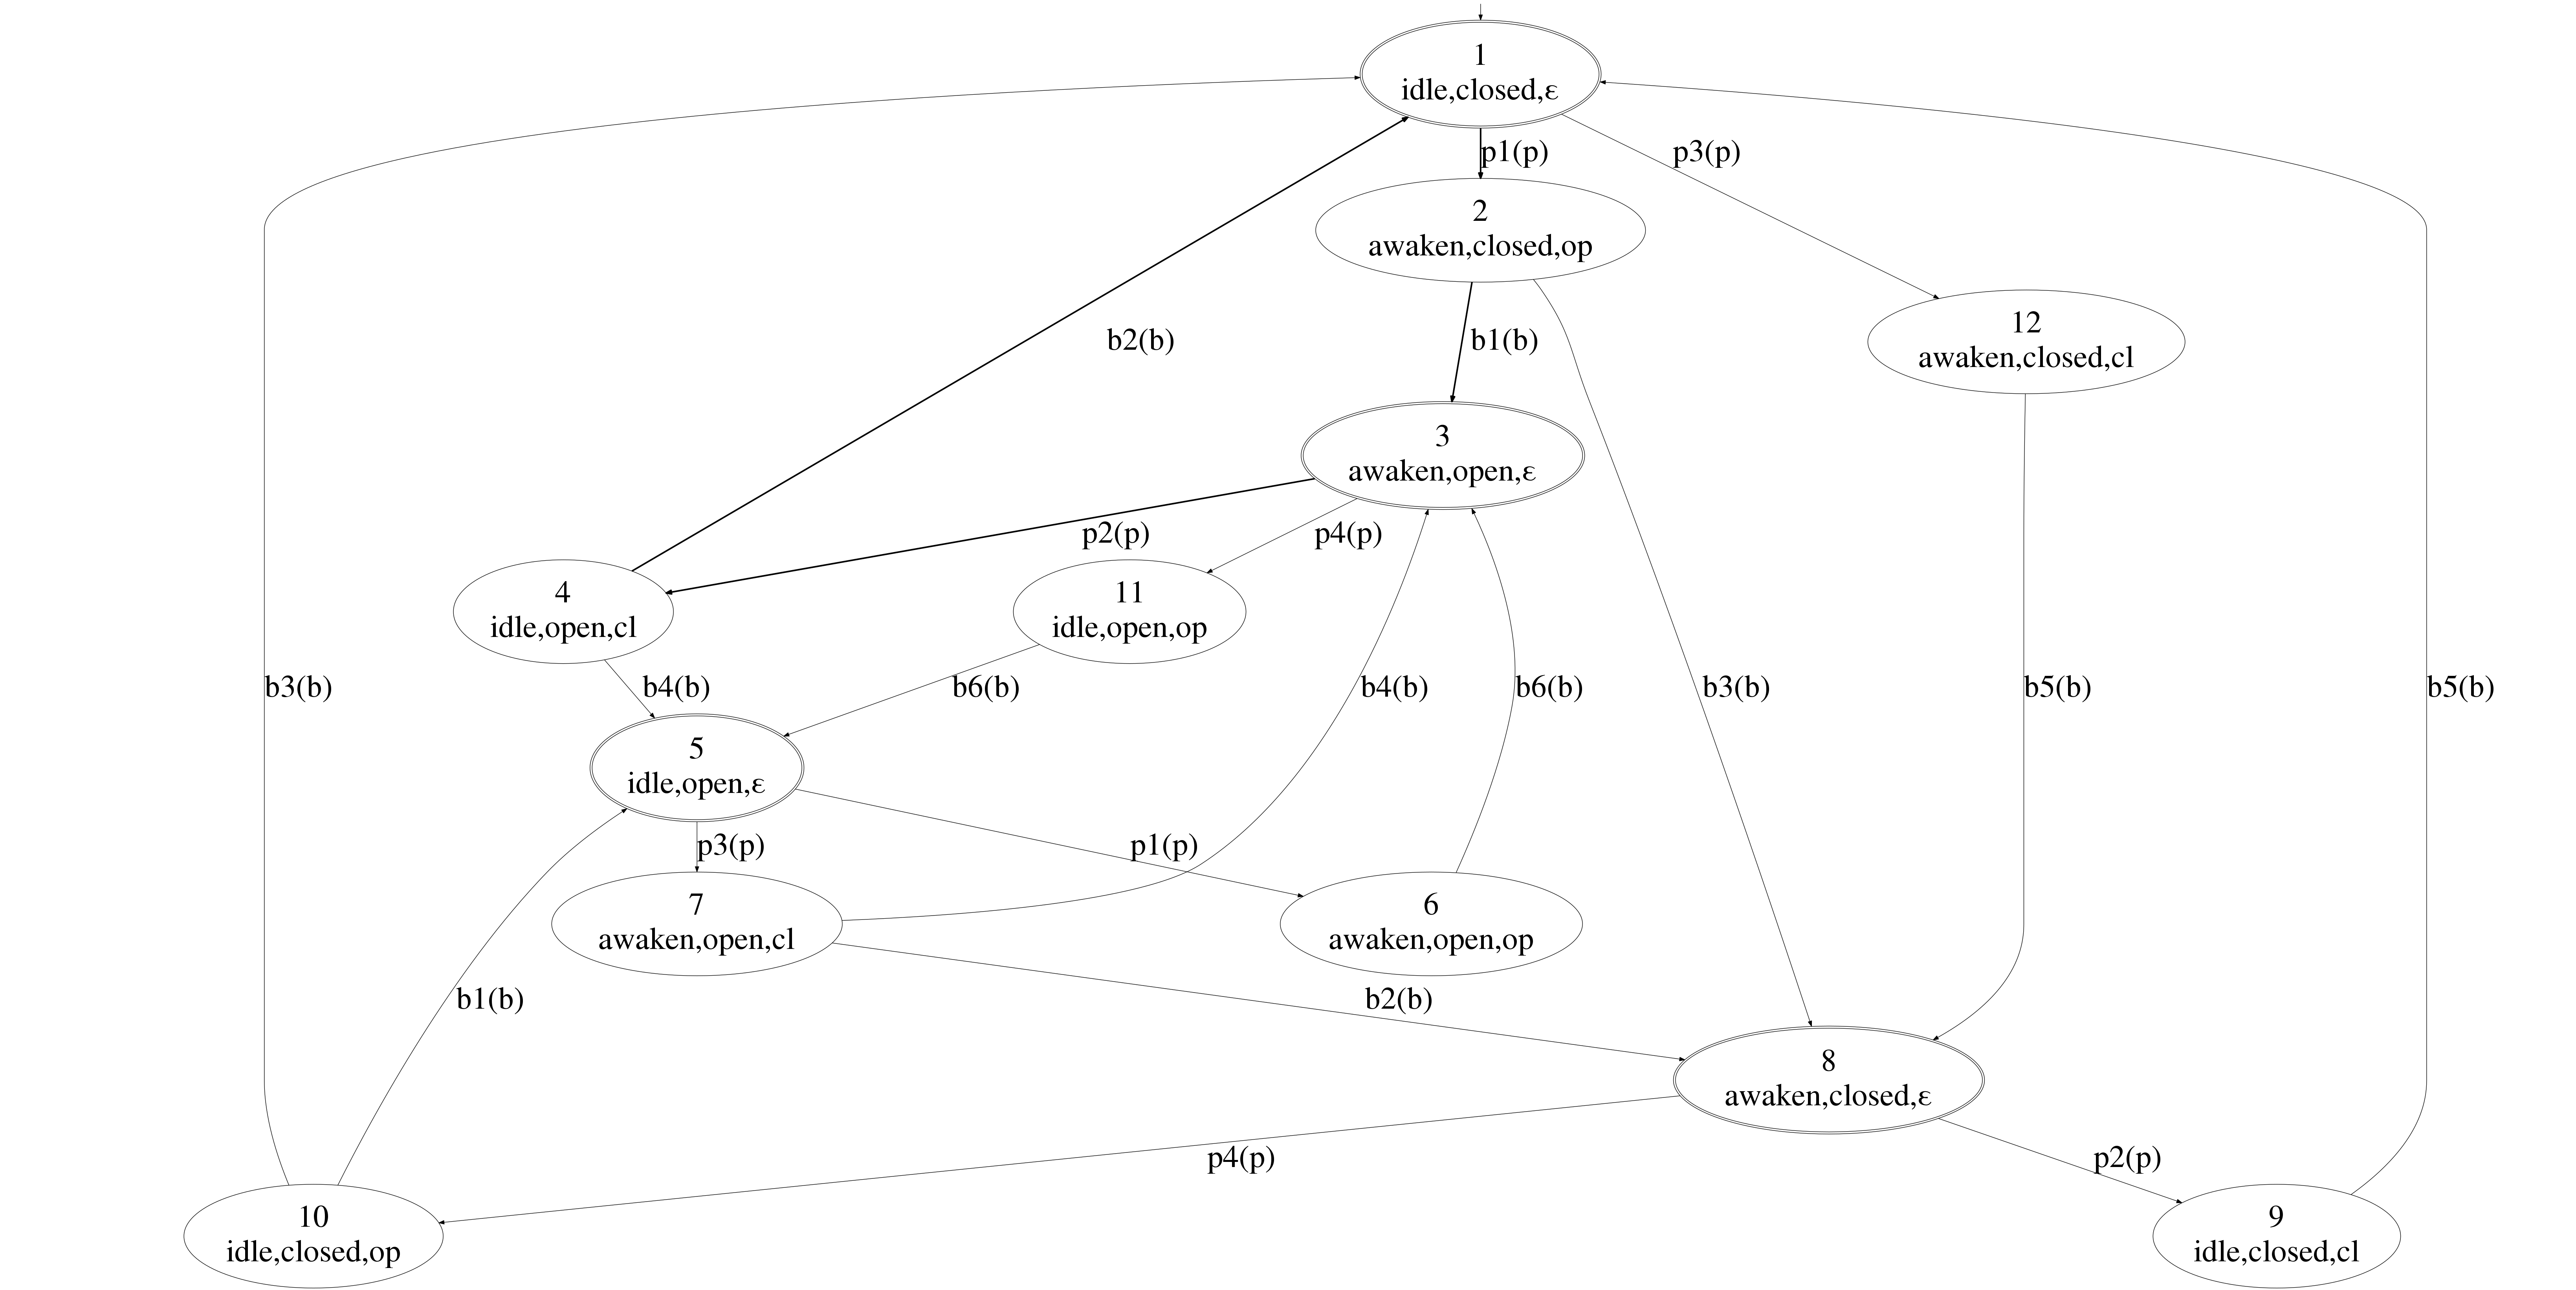
\includegraphics[scale=0.11]{./Img/sa/behavior_space.png}
\caption{Behavior space del sistema attivo $\overline{A}$}
\label{fig:bsp}
\end{figure}

\newpage
\section{Problema di diagnosi}
Un sistema attivo, inizialmente, si trova in uno stato quiescente, ovvero in uno stato in cui i link sono vuoti. Il sistema passa alla fase reattiva nel momento in cui riceve dei particolari eventi esterni. Una volta che l'occorrenza di un tale evento si verifica, la reazione del sistema è composta da una sequenza di transizioni che formano una traiettoria. Dato che ogni componente è modellato dal suo comportamento completo, ovvero sia dai suoi comportamenti normali sia quelli di guasto, sono necessarie delle informazioni aggiuntive, in grado di determinare se le transizioni facenti parte della traiettoria siano di guasto o normali. Un ulteriore problema consiste nella non completa osservabilità tipica dei sistemi reali: una traiettoria, in generale, non è percepita come effettivamente è, ma quello che è visibile consiste in una proiezione di un suo sottoinsieme osservabile. Una sequenza di label osservabili costituisce una traccia della reale traiettoria. Inoltre, una label associata ad una transizione di un componente potrebbe non identificare univocamente la transizione, poiché più transizioni possono condividere la medesima label di osservazione. Si noti come i modelli comportamentali dei singoli componenti non effettuino una distinzione tra ciò che osservabile e quello che non lo è: per questo motivo è necessaria una specifica esplicita di questa informazione. Una ulteriore componente significativa del problema è l'osservazione, solo a seguito della quale può essere formulata una diagnosi. Un'osservazione consiste in una sequenza di label osservabili.

\subsection{Viewer}
Una transizione è osservabile se, in corrispondenza della sua esecuzione, genera una label osservabile, altrimenti la transizione è non osservabile. La specifica dell'osservabilità di un sistema attivo è una corrispondenza tra transizioni (osservabili) e rispettive label.
\begin{defn}
Sia $A$ un sistema attivo e $\Omega$ un dominio di label osservabili. Un viewer $V$ di $A$ è una funzione suriettiva da un sottoinsieme di transizioni di componenti a $\Omega$.
\end{defn}
Si noti che, dal momento che la funzione di osservabilità è suriettiva, possono esservi più transizioni che vengono mappate nella stessa label. Questo aspetto è dovuto alla limitata osservabilità di un sistema così caratterizzato.

\begin{defn}
Sia $h$ una traiettoria di un sistema attivo $A$, e $V$ un viewer per $A$. La traccia di $h$ basata su $V$, scritta $h_{[V]}$, è la sequenza di etichette osservabili:
\begin{center}
$h_{[V]} = \{l|t \in h, (t,l) \in V\}$
\end{center}
\end{defn}
In altre parole, la traccia di una traiettoria $h$ di un sistema attivo è la proiezione delle transizioni osservabili di $h$ nelle corrispondenti label osservabili definite nel viewer $V$.

\begin{ex}
In tabella \ref{tab:viewer} è rappresentato un possibile \emph{viewer} per il sistema attivo $\overline{A}$ dell'esempio \ref{ex:sa}. Si noti che le uniche transizioni osservabili del breaker sono $b_1$ e $b_2$. Per quanto riguarda la protezione, nonostante tutte le transizioni siano osservabili, la stessa etichetta $awk$ è associata alle transizioni $p_1$ e $p_3$, mentre la label $ide$ è associata alle transizioni $p_2$ e $p_4$. 
\end{ex}

\begin{table}[htbp] 
\begin{tabularx}{\textwidth}{l X X X X X X X X X X}
\hline
\textbf{Transizione} & $p_1$ & $p_2$ & $p_3$ & $p_4$ & $b_1$ & $b_2$ & $b_3$ & $b_4$ & $b_5$ & $b_6$\\
\hline
\textbf{Label osservabile} & $awk$ & $ide$ & $awk$ & $ide$ & $opb$ & $clb$ &  &  &  & \\
\hline
\end{tabularx}
\caption{\emph{Viewer} per il sistema attivo $\overline{A}$}
\label{tab:viewer}
\end{table}

\subsection{Osservazione temporale}
L'osservazione temporale di un sistema attivo è una sequenza di label osservabili, dunque una traccia.
Si noti che ad una stessa traccia possono corrispondere più traiettorie, a causa della presenza di transizioni non osservabili.

\begin{ex} \label{ex:oss}
Con riferimento all'esempio \ref{ex:sa} e al \emph{viewer} definito nella tabella \ref{tab:viewer}, una possibile osservazione del sistema attivo $\overline{A}$ è la seguente:
\begin{center}
$\overline{O} = [ awk, opb, ide] $
\end{center}
\end{ex}


\subsection{Ruler}
La distinzione tra comportamento normale e difettoso viene fornita esplicitando quali, tra le transizioni dei componenti, sono corrette e quali di guasto. In questo modo una transizione $a \xrightarrow{t(c)} a^\prime$ di $A$ è di guasto se e solo se la transizione $t$ del componente $c$ è di guasto.
L'informazione che permette di individuare i guasti è fornita dal ruler.
\begin{defn}
Sia $A$ un sistema attivo e $\Phi$ un dominio di etichette di guasto. Un ruler $R$ per $A$ è una funzione, in generale suriettiva, da un sottoinsieme di transizioni di componenti a $\Phi$.
\end{defn}
Si noti che, per convenienza, la funzione di mapping potrebbe essere biettiva; tuttavia alcune transizioni di guasto possono non essere distinte le une dalle altre, in base al livello di precisione che si vuole dare alla diagnosi. Per esempio, due o più transizioni di guasto relative allo stesso componente possono essere mappate nella medesima label di guasto: in questo modo la diagnosi rileverà un generico guasto al componente, che in alcuni casi reali può essere una informazione sufficiente.
Si noti che la specifica del ruler viene data posteriormente al modello del sistema. Questo perché, in linea generale, differenti problemi di diagnosi, anche legati allo stesso sistema, possono essere caratterizzati da ontologie diverse, ognuna delle quali con un particolare modo di specificare le transizioni di guasto e le relative label. Un approccio ibrido, che è quello utilizzato in questo lavoro di tesi (esteso al caso di sistemi attivi complessi), consiste nel definire opzionalmente un ruler in fase di modellazione, fornendo la possibilità di ridefinirlo nella successiva diagnosi.

\begin{ex}
In tabella \ref{tab:ruler} è rappresentato un possibile \emph{ruler} per il sistema attivo $\overline{A}$ dell'esempio \ref{ex:sa}. La protezione ha come etichette di guasto $fop$, che si verifica quando la transizione $p_3$ fallisce nel comandare l'apertura del breaker, e $fcp$, che si verifica quando la transizione $p_4$ fallisce nel comandare la chiusura del breaker. 
Il breaker è caratterizzato da due guasti: la label $nob$ si riferisce alla mancata apertura del breaker nella transizione $b_3$, mentre $ncb$ alla sua mancata chiusura nella transizione $b_4$.
\end{ex}

\begin{table}[htbp] 
\begin{tabularx}{\textwidth}{l X X X X X X X X X X}
\hline
\textbf{Transizione} & $p_1$ & $p_2$ & $p_3$ & $p_4$ & $b_1$ & $b_2$ & $b_3$ & $b_4$ & $b_5$ & $b_6$\\
\hline
\textbf{Label di guasto} &  &  & $fop$ & $fcp$ &  &  & $nob$ & $ncb$ &  & \\
\hline
\end{tabularx}
\caption{\emph{Ruler} per il sistema attivo $\overline{A}$}
\label{tab:ruler}
\end{table}

\begin{defn}
Sia $h$ una traiettoria di un sistema attivo $A$, e $R$ un ruler per $A$. La diagnosi di $h$ basata su $R$, scritta $h_{[R]}$, è l'insieme delle label di guasto:
\begin{center}
	$h_{[R]} = \{ f | t \in h, (t,f) \in R \}$.
\end{center}
\end{defn}

\begin{ex}
Con riferimento all'esempio \ref{ex:sa}, si consideri la traiettoria:
\begin{center}
$h = [p_1,b_1,p_4,b_6]$
\end{center} 
In base al \emph{ruler} $\overline{R}$ definito nella tabella \ref{tab:ruler}, la diagnosi della traiettoria $h$ è l'insieme $h_{[\overline{R}]} = \{fcp\}$, ottenuto dal guasto in corrispondenza della transizione $p_4$.
\end{ex}

\subsection{Problema di diagnosi}
\begin{defn}
Sia $A$ un sistema attivo, $V$ un viewer di $A$, $O$ una osservazione temporale per $A$ relativa ad una traiettoria che parte dallo stato $a_0$, e $R$ un ruler per $A$. La quadrupla
\begin{center}
	$P(A) = (a_0,V,O,R)$
\end{center}
è un problema di diagnosi per $A$.
\end{defn}
Concettualmente, è possibile definire la soluzione di un problema di diagnosi nel seguente modo.
\begin{defn}
Sia $P(A) = (a_0,V,O,R)$ un problema di diagnosi per il sistema attivo $A$, e $Bsp(A)$ il behavior space con stato iniziale $a_0$. La soluzione del problema di diagnosi $\Delta(P(A))$, è l'insieme di diagnosi:
\begin{center}
	$\Delta(P(A)) = \{ \delta | \delta = h_{[R]}, h \in Bsp(A), h_{[V]} = O\}$
\end{center}
\end{defn}
In altre parole, la soluzione di un problema di diagnosi è l'insieme costituito dagli insiemi di guasti rilevati lungo le traiettorie la cui traccia è consistente con l'osservazione temporale.

\begin{ex} \label{ex:problem}
Si consideri il \emph{behavior space} del sistema attivo $\overline{A}$ in figura \ref{fig:bsp}, l'osservazione dell'esempio \ref{ex:oss} $\overline{O} = [awk, opb, ide]$, il viewer $\overline{V}$ e il ruler $\overline{R}$ riportati rispettivamente nelle tabelle \ref{tab:viewer} e \ref{tab:ruler}.
Le possibili traiettorie consistenti con l'osservazione sono:
\begin{itemize}
\item $h_1 = [p_1,b_1,p_2,b_4]$, a cui corrisponde la diagnosi $h_{1,[\overline{R}]} = \{ncb\}$;
\item $h_2 = [p_1,b_1,p_4,b_6]$, a cui corrisponde la diagnosi $h_{2,[\overline{R}]} = \{fcp\}$.
\end{itemize}
La soluzione del problema di diagnosi $P(\overline{A}) = (a_0,\overline{V},\overline{O},\overline{R})$ è data dalla composizione delle diagnosi di queste traiettorie:
\begin{center}
$\Delta(P(\overline{A}) = \{\{ncb\},\{fcp\}\}$.
\end{center}
Il significato delle due soluzioni trovate è il seguente: o il breaker $b$ non riesce a chiudersi, oppure la protezione $p$ invia il comando sbagliato al breaker.  
\end{ex}


\newpage
\section{Diagnosi monolitica}
La soluzione di un problema di  diagnosi, presentata nella sezione precedente, è definita come l'insieme delle label di guasto che vengono generate dalle traiettorie consistenti con l'osservazione temporale. Questa definizione, tuttavia, non presenta una tecnica che permetta di trovare tale insieme nella pratica, anche perché si suppone che il \emph{behavior space} non sia disponibile per la diagnosi. Scopo di questo paragrafo è quello di fornire, a fronte della definizione vista in precedenza, un metodo efficace che permetta di ottenere l'insieme delle diagnosi candidate in modo corretto e completo. 
Come prima osservazione, è essenziale notare che per generare le diagnosi candidate bisogna analizzare le traiettorie del sistema che sono consistenti con l'osservazione temporale. Per fare questo, bisogna poter generare un sotto-automa del behavior space contenente le sole traiettorie consistenti con l'osservazione temporale. 
La prima fase della diagnosi monolitica consiste nella costruzione del behavior $Bhv$, il cui linguaggio coincide esattamente con il sottoinsieme del linguaggio del behavior space consistente con l'osservazione temporale. Successivamente è necessario associare ad ogni traiettoria del behavior la corrispondente diagnosi. Questa procedura potrebbe essere infinita, dato che un automa può avere ciclicità e quindi dare luogo ad un insieme infinito di traiettorie. Tuttavia, è bene notare come l'insieme delle diagnosi è sempre finito, poiché limitato superiormente dal numero di label di guasto specificate nel ruler: nello specifico, l'insieme delle diagnosi è un sottoinsieme di $2^\Phi$, cioè l'insieme potenza del dominio di label di guasto $\Phi$. Nella pratica, l'insieme finito di traiettorie da considerare sono tutte quelle in cui i cicli sono attraversati al massimo una volta. Questo perché percorrere un ciclo più di una volta non cambia le diagnosi, dato che quelle ivi presenti sono già state collezionate durante l'iterazione precedente del ciclo.
Il secondo punto della diagnosi monolitica consiste nel generare l'insieme di diagnosi associate ad ogni nodo del behavior, ovvero praticare la cosiddetta decorazione del behavior.
Una volta che il behavior è stato costruito e decorato, l'ultima fase della diagnosi monolitica prevede la distillazione delle diagnosi, compiuta selezionando unicamente le diagnosi delle traiettorie consistenti con l'osservazione temporale. Per fare questo è importante distinguere, nella costruzione del behavior, tra stati finali e stati non finali. Uno stato del behavior è finale se e solo se tutte le traiettorie che giungono in quello stato hanno consumato interamente l'osservazione, cioè hanno percorso delle transizioni le cui label osservabili hanno prodotto una sequenza pari a quella dell'osservazione data. 

\subsection{Ricostruzione del behavior}
Il primo passo della diagnosi monolitica consiste nella ricostruzione del behavior. 
\begin{defn}
Sia $P(A) = (a_0,V,O,R)$ un problema di diagnosi per un sistema attivo $A = (C,L,D)$, dove $C$ è un insieme di $n$ componenti, mentre $L$ è un insieme di $m$ link. Sia $I(O)$ la sequenza di indici $[0 \ldots i_f]$ che rappresentano la consumazione dell'osservazione di lunghezza $i_f$ del sistema, con $0$ che rappresenta l'indice corrispondente all'osservazione iniziale nulla. Il behavior spurio di $P(A)$ è l'automa deterministico
\begin{center}
	$Bhv^s(P(A)) = (\Sigma,B^s,\tau^s,\beta_0,\beta_f)$
\end{center}
dove:
\begin{enumerate}
\item $\Sigma$ è l'alfabeto, costituito dall'unione delle transizioni dei componenti in $C$;
\item $B^S$ è l'insieme di stati $(S,Q,i)$, con $S = (s_1,\ldots,s_n)$ la n-pla di stati di tutti i componenti in $C$, $Q = (q_1,\ldots,q_m)$ la m-pla del contenuto di tutti i link in $L$, e $i$ l'indice corrente della sequenza di osservazione;
\item $\beta_0 = (S_0,Q_0,0)$ è lo stato iniziale, dove $a_0 = (S_0,Q_0)$ e $0$ è l'indice dell'osservazione iniziale nulla;
\item $\beta_f$ è l'insieme degli stati finali $(S_f,Q_f,i_f)$, dove $i_f$ è l'indice finale della sequenza di osservazione e $Q_f = \{\epsilon, \ldots, \epsilon\}$, ovvero tutti i link devono essere vuoti;
\item $\tau^s$ è la funzione di transizione, $\tau^s: B^s \times \Sigma \rightarrow B^s$, dove $(S,Q,i) \xrightarrow{t(c)} (S^\prime,Q^\prime,i^\prime) \in \tau^s$ e 
\begin{center}
	$t(c) = s \xrightarrow{(e,x) | \{(e_1,y_1), \ldots, (e_p,y_p)\}} s^\prime$
\end{center}
con $e$ disponibile in corrispondenza del terminale di input $x$, oppure nullo se rappresenta un evento esterno o relativo ad un terminale scollegato in $D_{on}$. La transizione è effettuabile se e solo se:
\begin{itemize}
\item Per ogni $j \in [1 \ldots n]$:
\begin{center}
$s^\prime_j = \begin{cases} s^\prime & \mbox{se }c_j = c\\ s_j & \mbox{altrimenti} \end{cases}$
\end{center}
cioè per ogni transizione del behavior space cambia lo stato relativo al singolo componente coinvolto nella transizione;
\item $Q^\prime$ differisce da $Q$ per le seguenti condizioni:
\begin{itemize}
\item $Q(x) = e \rightarrow Q^\prime(x) = \epsilon$, cioè l'evento in input è consumato;
\item $\forall(e_j,y_j), j \in [1 \ldots p], Q(y_j) = \epsilon \rightarrow Q^\prime(y_j) = e_j$, cioè gli eventi di uscita sono inseriti nei terminali di input connessi ai terminali di output coinvolti nella transizione; 
\end{itemize}
\item nel caso $t(c)$ sia osservabile, essa è presente nel viewer $V$ associata alla label $l$ e quest'ultima è una label contenuta nella sequenza di osservazione $O$ in corrispondenza dell'indice $i+1$, successivo a quello corrente. In questo caso l'indice dell'osservazione deve essere aggiornato ($i^\prime = i+1$). Nel caso invece $t(c)$ non sia osservabile, l'indice dell'osservazione rimane immutato ($i^\prime = i$).
\end{itemize}
\end{enumerate}

\end{defn}
Il behavior $Bhv(P(A)) = (\Sigma,B,\tau,\beta_0,\beta_f)$ è ottenuto rimuovendo dal behavior spurio tutti gli stati e tutte le transizioni che non appartengono a nessun cammino tra lo stato iniziale e uno degli stati finali (operazione di trim).
La definizione di behavior è ottenuta dalla definizione di behavior space, secondo le seguenti variazioni:
\begin{enumerate}
\item ogni stato del behavior include un campo aggiuntivo, l'indice $i$ della sequenza di osservazione;
\item la funzione di transizione richiede un requisito aggiuntivo di consistenza con l'osservazione temporale, nel caso la transizione sia osservabile;
\item nel behavior gli stati finali, oltre ad avere tutti i link vuoti, indicano il raggiungimento della completa consumazione della sequenza osservata;
\item nel passaggio dal behavior spurio al behavior, sono mantenuti solo gli stati e le transizioni incluse in un cammino dallo stato iniziale ad uno stato finale.
\end{enumerate}
Secondo le definizioni viste in precedenza, quindi, il linguaggio del behavior costituisce un sottoinsieme del linguaggio del behavior space, in quanto costituito unicamente da quelle traiettorie che sono consistenti con l'osservazione temporale.
Di seguito è riportato lo pseudocodice dell'algoritmo di ricostruzione del behavior (\ref{alg:bhv}), in accordo con la definizione.

\begin{algorithm}
\textbf{BuildBhv($P(A) = (a_0,V,O,R)$)}
\begin{algorithmic}
	\STATE $\beta_0 \leftarrow (S_0,Q_0,0)$, dove $a_0 = (S_0,Q_0)$
	\STATE $B \leftarrow \{\beta_0\}$
	\STATE $\tau \leftarrow \emptyset$
	\REPEAT
		\STATE Viene scelto uno stato non ancora marcato $\beta = (S,Q,i)$
		\FORALL{$t(c)$ effettuabile in $\beta$} 
			\IF{$t(c)$ non è osservabile in $V$}
				\STATE $i^\prime \leftarrow i$
			\ELSIF{$t(c)$ è osservabile in $V$ tramite la label $l$ \AND $l \in O$ in corrispondenza dell'indice $i+1$}
				\STATE $i^\prime \leftarrow i+1$
			\ELSE
				\STATE continue
			\ENDIF
			\STATE $S^\prime \leftarrow S$ e viene aggiornato lo stato del componente $c$ di $t(c)$
			\STATE $Q^\prime \leftarrow Q$ e viene aggiornato lo stato dei link coinvolti in $t(c)$
			\STATE $\beta^\prime \leftarrow (S^\prime,Q^\prime,i^\prime)$
			\IF{$\beta^\prime \notin B $}
				\STATE $\beta^\prime$ è inserito in $B$
			\ENDIF
			\STATE La transizione $\beta \xrightarrow{t(c)} \beta^\prime$ è inserita in $\tau$
		\ENDFOR
		\STATE Lo stato $\beta$ è marcato
	\UNTIL{tutti gli stati in $B$ sono marcati}
	\STATE $\beta_f \leftarrow \{\beta_f | \beta_f \in B, \beta_f=(S,Q,i_f), i_f$  indice finale di $O\}$
	\STATE Rimuovere da $B$ e da $\tau$, rispettivamente, tutti gli stati e le transizioni non inclusi in un cammino da $\beta_0$ ad uno stato finale
\end{algorithmic}
\caption{Algoritmo di ricostruzione del behavior}
\label{alg:bhv}
\end{algorithm}

\begin{ex}
Con riferimento al problema di diagnosi nell'esempio \ref{ex:problem} in figura \ref{fig:bhv} è riportato  il behavior del problema di diagnosi $P(\overline{A})$. Le transizioni e gli stati tratteggiati costituiscono la parte spuria dell'automa, in quanto non appartengono a nessun cammino dallo stato iniziale a uno stato finale. Uno stato è finale se, oltre ad avere i link vuoti, ha un indice di osservazione pari a $3$, che costituisce l'indice finale della sequenza di osservazione $\overline{O} = [awk,opb,ide]$ di lunghezza $3$.
Si noti la differenza di questo automa con il behavior space della figura \ref{fig:bsp}. 
La diversa grandezza degli automi può essere evidenziata meglio in sistemi attivi con un numero maggiore di componenti e link, a causa della crescita esponenziale degli automi.
\end{ex}

\begin{figure}[htbp]
\centering
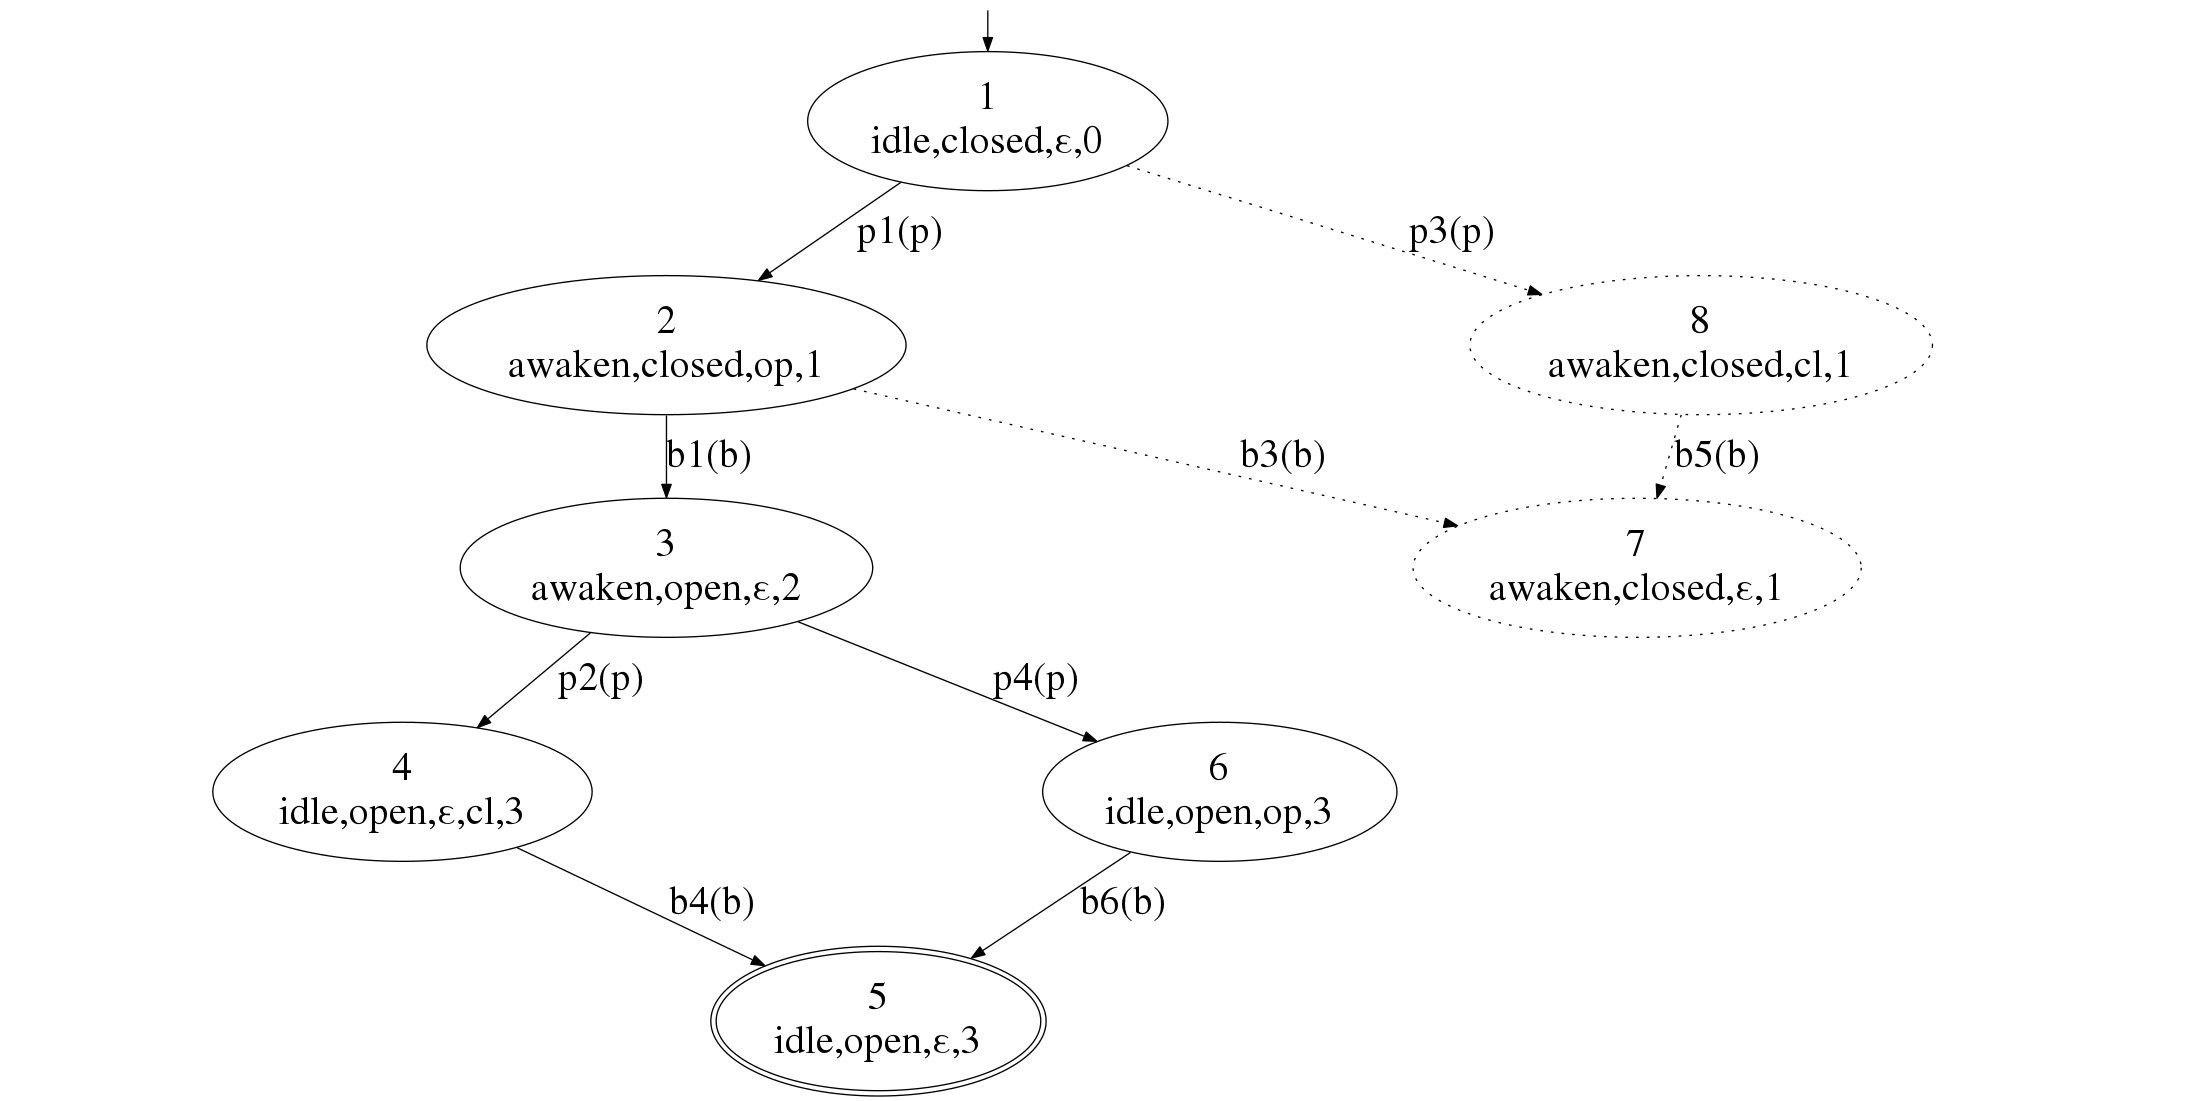
\includegraphics[scale=0.15]{./Img/sa/bhv_s.png}
\caption{Behavior del problema di diagnosi $P(\overline{A})$. Le transizioni e gli stati tratteggiati indicano la parte spuria dell'automa}
\label{fig:bhv}
\end{figure}

\subsection{Decorazione del behavior}
Il secondo passo della ricostruzione monolitica consiste nella decorazione del behavior. Il linguaggio dell'automa ottenuto nel passo precedente è composto da stringhe, ognuna delle quali rappresenta una traiettoria consistente con l'osservazione temporale. Dato che il behavior racchiude tutte e sole le traiettorie la cui traccia rispetto al viewer è una traccia candidata dell'osservazione, la soluzione del problema di diagnosi è l'insieme delle diagnosi relative a tali traiettorie. Dato che le traiettorie potrebbero avere dei cicli, dando luogo ad un numero infinito di percorrenze, l'idea è quella di marcare ogni stato del behavior con l'insieme di diagnosi relative a tutte le traiettorie che terminano in quello stato. Il fatto di avere ciclicità non è un problema, poiché la percorrenza di più cicli non accresce la diagnosi già collezionata in precedenza. Il processo di marcare ogni stato con le relative diagnosi è detto decorazione.

\begin{defn}
Sia $Bhv(P(A))$ il behavior di un problema di diagnosi $P(A)$. Il behavior decorato $Bhv^\star(P(A))$ è il DFA ottenuto dal behavior marcando ogni stato $\beta$ con un insieme di diagnosi $\Delta(\beta)$ basato sull'applicazione delle seguenti regole:
\begin{enumerate}
\item lo stato iniziale è decorato con l'insieme di diagnosi vuoto $\delta(\beta_0) = \{\emptyset\}$
\item per ogni transizione $\beta \xrightarrow{t(c)} \beta^\prime$, per ogni $\delta \in \Delta(\beta)$, se $(t(c),f) \in R$ allora $\delta \cup \{f\} \in \Delta(\beta^\prime)$, altrimenti $\delta \in \Delta(\beta^\prime)$.
\end{enumerate}
\end{defn}
La prima regola è quella base, in cui si associa alla traiettoria nulla la diagnosi vuota.
Se la decorazione di uno stato $\beta$ include una diagnosi $\delta$ allora esiste almeno una traiettoria $h$, che termina in $\beta$, la cui diagnosi è $\delta$. Conseguentemente, esiste una traiettoria $h \cup [t(c)]$ terminante in $\beta^\prime$ la cui diagnosi è $\delta$ se $(t(c),f) \notin R$, oppure è l'estensione di $\delta$ tramite la label di guasto $f$, associata alla transizione $t(c)$ nel ruler $R$. 
Quest'ultima regola è induttiva e deve essere applicata continuamente allo stato successivo della transizione fino a che la decorazione non aggiunge nuove diagnosi, raggiungendo una condizione di stabilità.
L'algoritmo di decorazione, in forma ricorsiva, è fornito di seguito (\ref{alg:decoration}).

\begin{algorithm}
\textbf{Decorate($Bhv(P(A))$)}
\begin{algorithmic}
\STATE Marcare lo stato iniziale $\beta_0$ con $\{\emptyset\}$ 
\STATE Marcare tutti gli altri stati non iniziali con l'insieme vuoto $\emptyset$
\STATE $Dec(\beta_0,\{\emptyset\})$
\STATE
\STATE \textbf{Function} $Dec(\beta$,$D)$
	\FORALL{transizione $\beta \xrightarrow{t(c)} \beta^\prime$}
		\STATE $D^+ \leftarrow \emptyset$
		\FORALL{$\delta \in D$}
			\IF{$(t(c),f) \in R$}
				\STATE $\delta^\prime \leftarrow \delta \cup \{f\}$
			\ELSE
				\STATE $\delta^\prime \leftarrow \delta$
			\ENDIF
			\IF{$\delta^\prime \notin \Delta(\beta^\prime)$}
				\STATE inserire $\delta^\prime$ in $\Delta(\beta^\prime)$ e in $D^+$
			\ENDIF
		\ENDFOR
		\IF{$D^+ \neq \emptyset$}
			\STATE $Dec(\beta^\prime, D^+)$
		\ENDIF
	\ENDFOR
\end{algorithmic}
\caption{Algoritmo di decorazione del behavior}
\label{alg:decoration}
\end{algorithm}

\begin{ex}
Con riferimento al problema di diagnosi dell'esempio \ref{ex:problem}, in figura \ref{fig:bhv_star} è rappresentato il relativo behavior decorato.
Nella tabella \ref{tab:decoration} sono riportate le chiamate effettuate dall'algoritmo alla procedura ricorsiva $Dec$. L'ordine di considerazione delle transizioni è, rispetto all'automa del behavior decorato, da sinistra a destra.
\end{ex}

\begin{figure}[htbp]
\centering
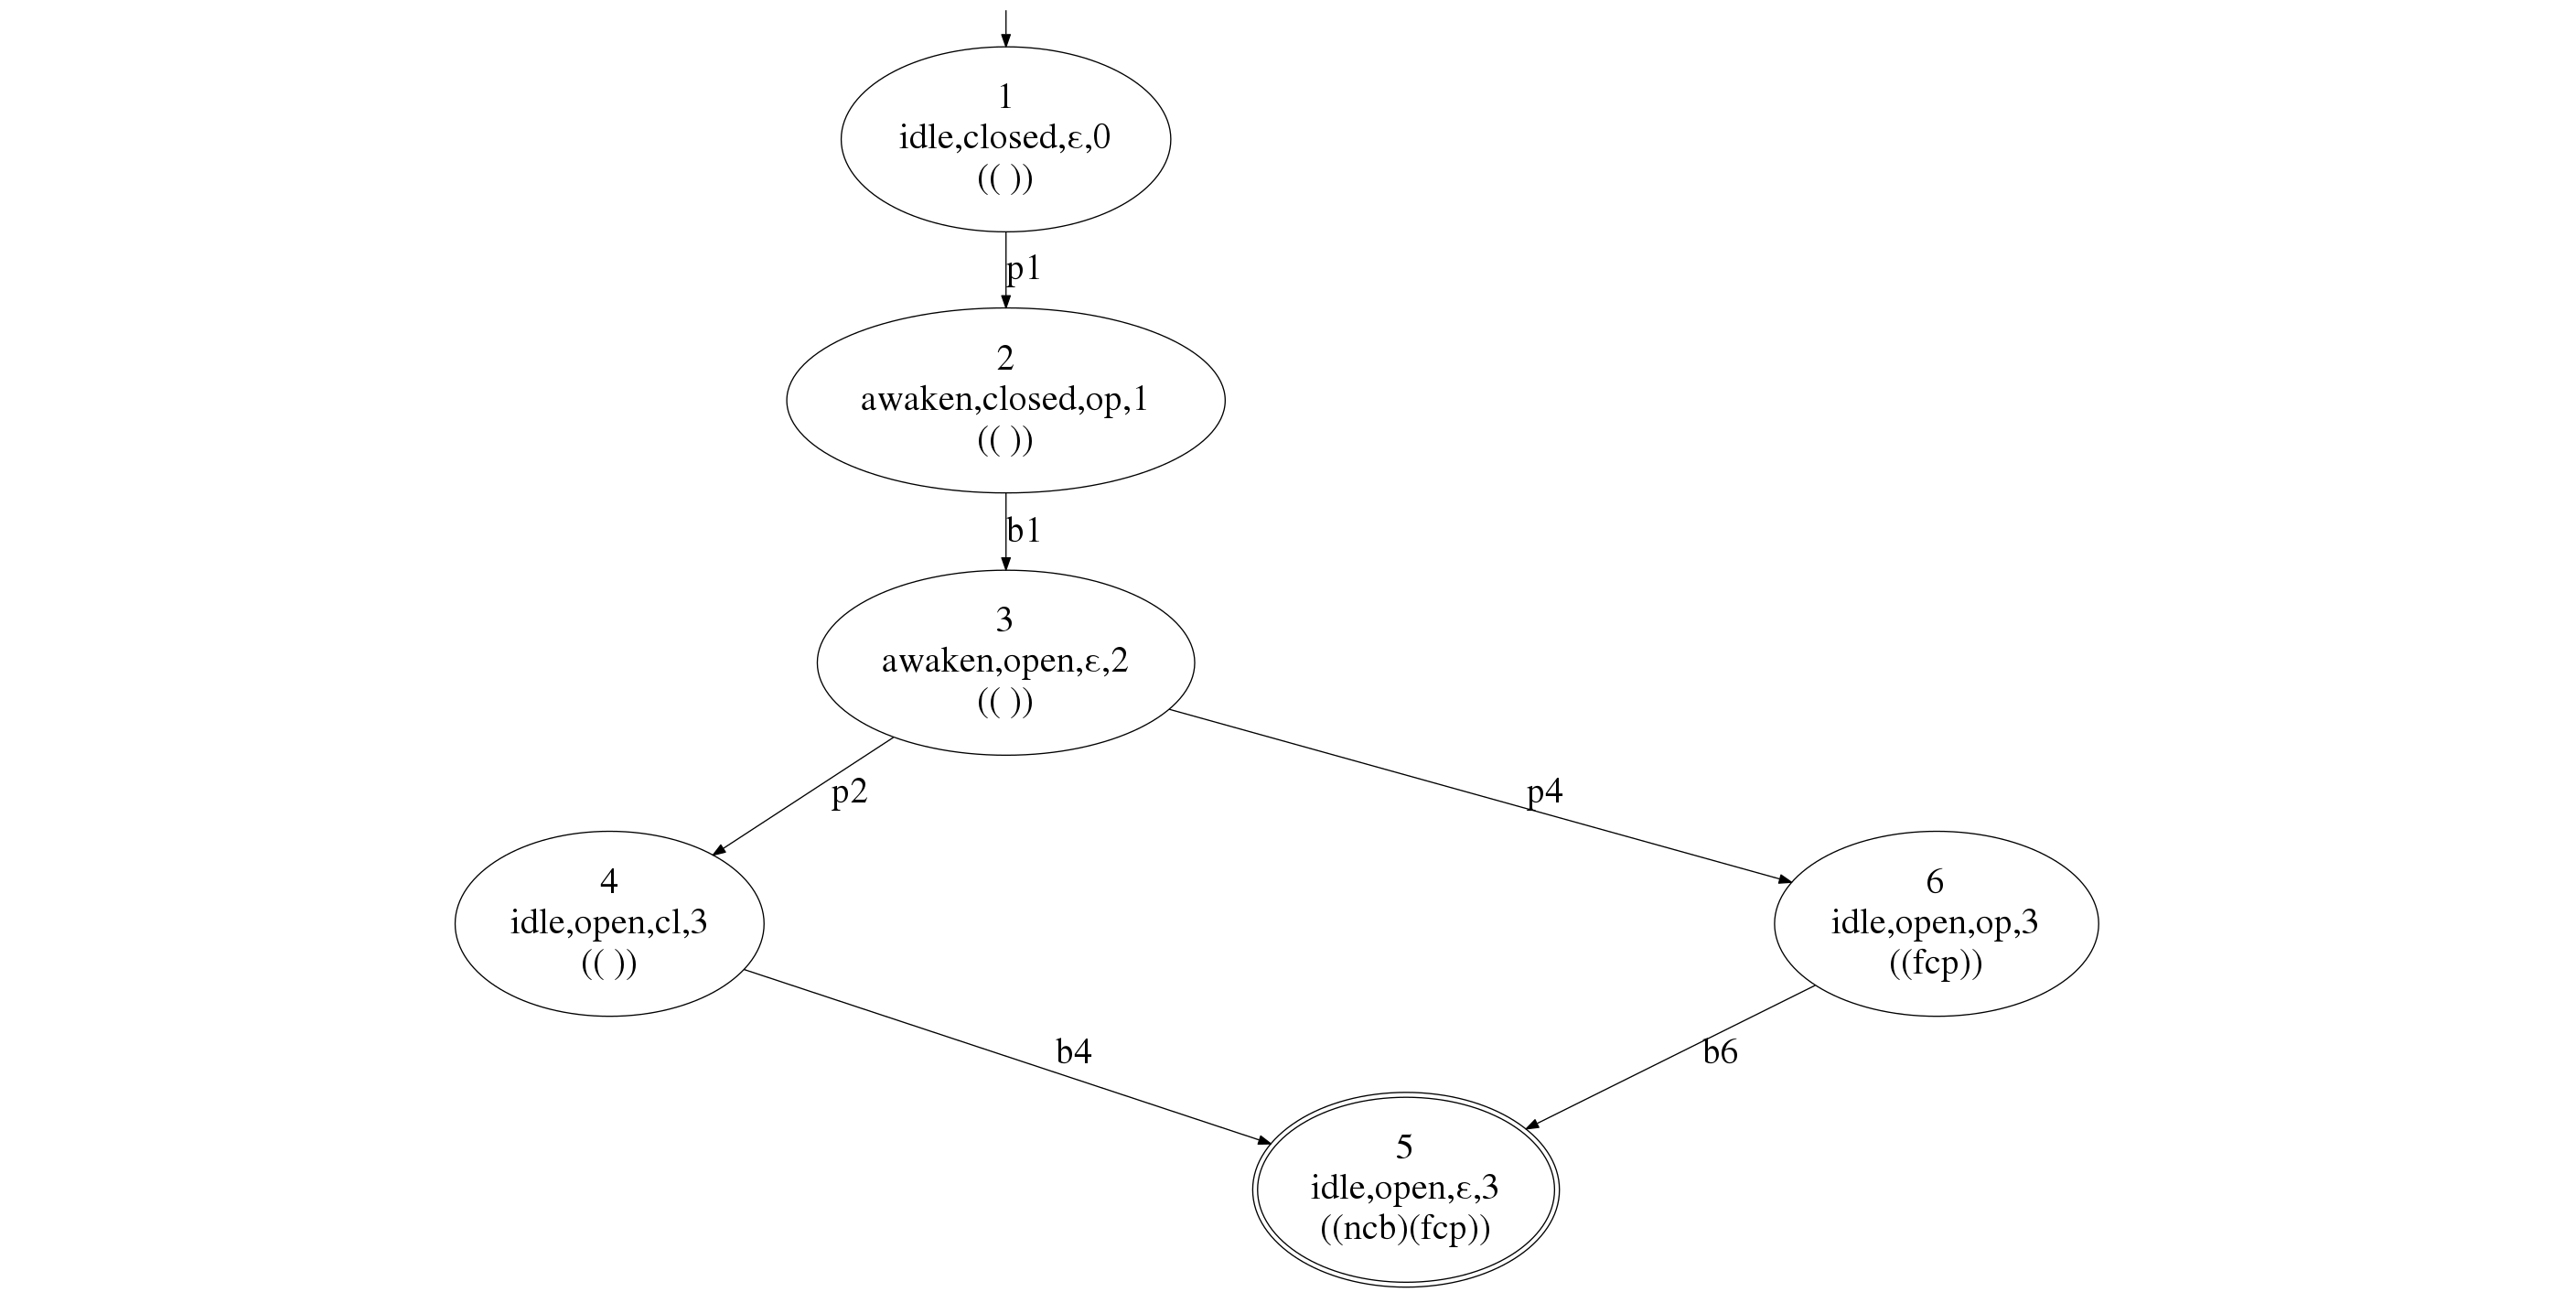
\includegraphics[scale=0.13]{./Img/sa/bhv_star.png}
\caption{Behavior decorato del problema di diagnosi $P(\overline{A})$}
\label{fig:bhv_star}
\end{figure}

\begin{table}[htbp] 
\begin{tabularx}{\textwidth}{l c c c c c c c}
\hline
N & Chiamata & $\Delta(1)$ & $\Delta(2)$ & $\Delta(3)$ & $\Delta(4)$ & $\Delta(5)$ & $\Delta(6)$\\
1 & $(1,\{\emptyset\})$ & $\{\emptyset\}$  & $\emptyset$ & $\emptyset$ & $\emptyset$ & $\emptyset$ & $\emptyset$\\
2 & $(2,\{\emptyset\})$ & $\{\emptyset\}$  & $\{\emptyset\}$ & $\emptyset$ & $\emptyset$ & $\emptyset$ & $\emptyset$\\
3 & $(3,\{\emptyset\})$ & $\{\emptyset\}$  & $\{\emptyset\}$ & $\{\emptyset\}$ & $\emptyset$ & $\emptyset$ & $\emptyset$\\
4 & $(4,\{\emptyset\})$ & $\{\emptyset\}$  & $\{\emptyset\}$ & $\{\emptyset\}$ & $\{\emptyset\}$ & $\emptyset$ & $\emptyset$\\
5 & $(5,\{\{ncb\}\})$ & $\{\emptyset\}$  & $\{\emptyset\}$ & $\{\emptyset\}$ & $\{\emptyset\}$ & $\{\{ncb\}\}$ & $\emptyset$\\
6 & $(6,\{\{fcp\}\})$ & $\{\emptyset\}$  & $\{\emptyset\}$ & $\{\emptyset\}$ & $\{\emptyset\}$ & $\{\{ncb\}\}$ & $\{\{fcp\}\}$\\
7 & $(5,\{\{fcp\}\})$ & $\{\emptyset\}$  & $\{\emptyset\}$ & $\{\emptyset\}$ & $\{\emptyset\}$ & $\{\{ncb\},\{fcp\}\}$ & $\{\{fcp\}\}$\\
\hline
\end{tabularx}
\caption{Applicazione dell'algoritmo di decorazione per ricavare $Bhv^\star(P(\overline{A}))$}
\label{tab:decoration}
\end{table}

\subsection{Distillazione delle diagnosi}
Una volta che il behavior è stato costruito e decorato, la soluzione del problema di diagnosi $P(A)$ può essere determinato calcolando l'unione delle diagnosi associate a stati finali del behavior decorato:
\begin{center}
$\Delta(P(A))) = \{\delta | \delta \in \Delta(\beta_f), \beta_f$ finale in $Bhv^\star(P(A))\}$.
\end{center}


\begin{ex}
Considerando il behavior decorato in figura \ref{fig:bhv_star}, la distillazione delle diagnosi avviene considerando l'insieme delle diagnosi relative all'unico stato finale $5$, cioè
\begin{center}
$\Delta(P(\overline{A})) = \{\{ncb\},\{fcp\}\}$
\end{center}
Si noti come la soluzione trovata è la stessa intuitivamente ricavata dalle definizioni nell'esempio \ref{ex:problem}.
\end{ex}
\chapter{Sistemi Attivi Complessi}
In questo capitolo vengono presentate definizioni e modelli che descrivono i sistemi attivi complessi, visti come estensione dei sistemi attivi tradizionali descritti precedentemente. Un sistema attivo complesso è una gerarchia di sistemi attivi tra loro comunicanti. Questo modello si ispira a molti sistemi naturali, fisici, economici e sociali, dei quali è possibile fornire un modello stratificato, in base a diversi livelli di astrazione. Nei sistemi biologici, ad esempio, il comportamento può essere descritto a basso livello dalle interazioni fra le cellule, oppure ad un livello più alto tra i tessuti, o ancora in maniera più astratta studiando il funzionamento degli organi. Nell'ambito dei linguaggi di programmazione a oggetti, ad esempio, a basso livello vi sono le singole istruzioni, a livello più alto i metodi, ad un più alto livello ancora le classi e le interfacce. 
L'attributo ``complesso'' si riferisce, più che alla quantità di componenti presenti nel sistema (che comunque possono essere molti), all'organizzazione gerarchica e alla conseguente stratificazione del comportamento globale del sistema.
Ogni livello della gerarchia di sistemi siffatti ha una evoluzione indipendente dagli altri, eccetto alcune informazioni che giungono dai livelli sottostanti. Ogni livello, in altre parole, ha un comportamento emergente che è impredicibile dalla semplice conoscenza del comportamento dei singoli componenti. Queste informazioni che giungono ai livelli superiori sono rese nel modello dei sistemi attivi complessi attraverso pattern event, che si verificano quando determinate configurazioni delle transizioni dei componenti sottostanti si verificano, soddisfacendo particolari espressioni regolari.

\newpage
\section{Definizioni}
Un sistema attivo complesso (SAC) è una gerarchia di sistemi attivi. In un SAC, vi sono due tipi di comunicazione: tra componenti dello stesso sistema attivo e tra differenti sistemi attivi. 
I componenti di un sistema attivo interagiscono tra loro in base a determinati eventi che giungono o da componenti adiacenti (eventi interni), o da altri sistemi attivi collegati (pattern event) o dal mondo esterno al sistema (eventi esterni). Questi eventi innescano delle transizioni nei componenti, le quali a loro volta generano nuovi eventi, formando una sequenza di transizioni detta traiettoria del SAC.
Analogamente ai sistemi attivi tradizionali, un sistema attivo complesso può essere in uno stato quiescente, nel quale nessun evento si verifica e conseguentemente non vengono innescate transizioni dei componenti.
Il SAC diviene reattivo nel momento in cui si verifica un evento esterno che può essere consumato da un componente. In tale circostanza la transizione di un componente modifica lo stato del sistema, dove lo stato è caratterizzato dalla composizione di tutti gli stati dei componenti, dagli eventi non ancora consumati presenti nei terminali di input, e dagli stati relativi agli automi (pattern space) responsabili del matching delle espressioni regolari generanti i pattern event. 

\subsection{Nodi}
Un sistema attivo complesso è composto da un insieme di sistemi attivi che interagiscono tra loro. Ogni singolo sistema attivo è detto nodo, in quanto costituisce un nodo nella gerarchia che costituisce la topologia del sistema.
Il modello di un nodo, a cui più istanze di nodi possono fare riferimento, possiede tutti gli attributi di un sistema attivo, con l'aggiunta di alcuni elementi:
\begin{itemize}
\item un insieme $I$ di terminali di input, nei quali giungono pattern event generati da nodi del livello inferiore;
\item un insieme $O$ di terminali di output, nei quali vengono generati i pattern event del nodo corrente, che vengono inviati a uno o più nodi del livello superiore;
\item un insieme $P$ di dichiarazioni di pattern;
\item un insieme $L_{patt}$ di link uscenti da terminali di input del nodo ed entranti in terminali di input dei componenti.
\end{itemize}
Quest'ultima caratteristica aggiuntiva consente l'invio dei pattern event in ingresso al nodo ai componenti particolari predisposti a gestire tali eventi.

\subsection{Pattern}
Una dichiarazione di pattern è una quadrupla $(p,l,r,o)$ dove:
\begin{itemize}
\item $p$ è il nome del pattern event;
\item $l$ è il linguaggio relativo al pattern;
\item $r$ è una espressione regolare;
\item $o \in O$ è un terminale di output in corrispondenza del quale il pattern event viene generato.
\end{itemize}
Il linguaggio $l$ del pattern può variare dal linguaggio minimo, cioè costituito dalle sole transizioni facenti parte dell'espressione regolare $r$, al linguaggio massimo, ovvero corrispondente all'insieme di tutte le transizioni di componenti del nodo. L'appartenenza a diversi linguaggi conferisce una semantica differente a quei pattern le cui espressioni regolari utilizzano operatori insiemistici, come ad esempio il $not$. Si nota facilmente che il complemento di una transizione rispetto a linguaggi differenti ha come risultato una unione di transizioni che, data l'operazione di complemento applicata su insiemi diversi, varia.

\subsection{Pattern space}
In modo da individuare pattern event, deve essere mantenuto lo stato relativo al matching dei pattern coinvolti. A tal fine, per ogni nodo, è necessario generare degli automi, chiamati \emph{pattern space}, secondo i seguenti passi:
\begin{itemize}
\item per ogni pattern $(p,l,r,o)$, viene generato un automa deterministico equivalente all'espressione regolare $r$, nel quale ogni stato finale viene marcato dal nome $p$ del pattern event;
\item per ogni linguaggio utilizzato nella definizione dei pattern, vengono identificati i pattern che utilizzano tale linguaggio, corrispondenti agli automi $[A_1, \ldots , A_k]$, e viene generato un pattern space nel seguente modo:
	\begin{enumerate}
	\item un automa non deterministico $N$ è creato generando il suo stato iniziale $s_0$ e una $\epsilon$-			transizione da $s_0$ a ogni stato iniziale di $A_i$, con $i \in [1 \ldots k]$;
	\item in modo da mantenere il matching di stringhe sovrapposte, viene aggiunta una $\epsilon$-transizione	da ogni stato non iniziale a $s_0$;
	\item l'automa $N$ viene determinizzato nel risultante pattern space $Pts$, dove ogni stato finale $s_f$ è marcato dall'unione \textbf{p} dei pattern event associati agli stati in $s_f$ che sono finali nei corrispondenti automi di pattern generati inizialmente. Ogni stato $s$ dell'automa deterministico $Pts$ è infatti identificato da un sottoinsieme di stati dell'automa non deterministico equivalente $N$.
	\end{enumerate}
\end{itemize}

\begin{ex}
Viene di seguito presentata la costruzione del pattern space relativo a due pattern (caratterizzati ovviamente dallo stesso linguaggio).
\end{ex}

\subsection{Link tra nodi}
Un sistema attivo complesso, oltre che da un insieme di nodi, è caratterizzato dalla topologia con cui i nodi sono collegati tra loro. Si assume che tale topologia generi un albero.
I nodi sono tra loro connessi per mezzo di link. I link tra nodi sono definiti analogamente ai link tra componenti del singolo sistema attivo, con la differenza che i primi connettono tra loro sistemi attivi.
In un SAC ogni link esce da un terminale di output $o$ di un nodo $n$ e entra in un terminale di input $i$ di un nodo $n^\prime$.
I link sono caratterizzati da un modello, che costituisce un'astrazione del link specifico in esame.

\begin{defn}
Un modello di un link è una quadrupla
\begin{center}
	$M_{l_c} = (i,o,z,w)$
\end{center}
dove $i$ è il terminale di input, $o$ il terminale di output, $z$ la dimensione e $w$ la politica di saturazione.
\end{defn}
Un particolare link $l_c$ è un'istanza di un modello siffatto, e consiste quindi in un canale di comunicazione unidirezionale fra due nodi del sistema $n$ e $n^\prime$, dove un terminale di output $o$ di $n$ e un terminale di input $i$ di $n^\prime$ coincidono rispettivamente con l'input e l'output del link $l_c$.
La dimensione $z$ rappresenta il numero massimo di eventi che possono essere accodati nel link. 
Indichiamo con $|l_c|$ la configurazione corrente del link. 
Se il numero di eventi attualmente memorizzati coincide con la dimensione, il link si dice essere saturo.
Quando il link è saturo, la semantica legata al compimento delle transizioni è dettata dalla politica di saturazione $w$ (si veda il paragrafo \ref{saturation}).
Come per i link tra componenti, anche per quanto riguarda i link tra nodi, nel seguito della trattazione, si farà riferimento al caso in cui la dimensione sia unitaria e la politica di saturazione sia $wait$.

\subsection{Sistema attivo complesso}
Un sistema attivo complesso è una rete di nodi interconnessi per mezzo di link. Ogni nodo ed ogni link del sistema sono caratterizzati da un modello e quindi, in generale, più elementi potrebbero avere il medesimo modello. Si assume che più link possano uscire da un terminale di output di un nodo, mentre al massimo un link possa entrare in un terminale di input.

\begin{defn}
Un sistema attivo complesso è una coppia
\begin{center}
	$ C = (N,L_c)$
\end{center}
dove $N$ è l'insieme di nodi, mentre $L_c$ è l'insieme dei link tra terminali di nodi appartenenti a $N$.
\end{defn}


\subsection{Traiettoria}
Un SAC può essere pensato come una macchina che può essere in uno stato quiescente o in uno stato reattivo. Se si trova nello stato quiescente, i componenti non effettuano alcuna transizione, dal momento che nessun evento è disponibile nei terminali di ingresso. In corrispondenza del verificarsi di un determinato evento proveniente dal mondo esterno, il sistema evolve nella sua fase reattiva. Dato che il comportamento del sistema è asincrono (non dipende dal tempo), la reazione, detta traiettoria (o storia), consiste in una sequenza di transizioni compiute da componenti presenti nel sistema.
Ogni transizione di un componente porta il sistema in un nuovo stato, dove uno stato è identificato dallo stato corrente di ogni componente di ogni nodo,dalle configurazioni attuali dei link dei nodi e dallo stato attuale dei pattern space di tutti i nodi. Quando un pattern space raggiunge uno stato finale, il relativo pattern event viene inviato al terminale corrispondente.
In altre parole, uno stato del sistema attivo complesso è una tripla $(S,Q,Pts)$, dove $S$ è la n-pla degli stati dei componenti dei nodi, $Q$ è la m-pla delle configurazioni dei link tra nodi, mentre $Pts$ è la p-pla di pattern space di tutti i nodi.
Quindi una transizione del sistema può essere scritta come:
\begin{center}
	$T = (S,Q,Pts) \xrightarrow {t(c(n))} (S^\prime,Q^\prime,Pts^\prime)$,
\end{center}
dove $t(c(n))$ identifica univocamente la transizione $t$ appartenente al modello del componente $c$ nel nodo $n$.
Assumendo che $a_0 = (S_0,Q_0,Pts_0)$ sia lo stato iniziale del sistema, la traiettoria ottenuta partendo da $a_0$ è la sequenza di stati del sistema determinata dall'occorrenza di transizioni $t_1, \ldots , t_k$ attuabili da parte dei singoli componenti dei nodi:
\begin{center}
$h = a_0 \xrightarrow{t_1(c_1(n_1))} a1 \xrightarrow{t_2(c_2(n_2))} a2 \ldots \xrightarrow{t_k(c_k(n_k))} a_k$.
\end{center}

Ogni stato (non iniziale) dipende quindi dallo stato precedente e dalla particolare transizione che lo porta allo stato corrente, ovvero la coppia $(a_{i-1},t_i(c_i(n_i)))$. Assumendo che si parta dallo stato iniziale $a_0$ questo ci permette di identificare una traiettoria per mezzo delle sole transizioni dei componenti dei nodi:
\begin{center}
$h = [t_1(c_1(n_1)),t_2(c_2(n_2)), \ldots , t_k(c_k(n_k))]$.
\end{center}


\subsection{Behavior space}
Dato un SAC $C$ ed il suo stato iniziale, possono esservi infinite traiettorie, descritte da un automa. 
Quest'ultimo è detto behavior space e ha come alfabeto l'intero insieme delle transizioni dei singoli componenti di ogni nodo.
Il linguaggio del behavior space $Bsp(C)$ con stato iniziale $a_0$ coincide con l'insieme di tutte le possibili traiettorie del sistema $C$ partendo dallo stato $a_0$. 
\begin{defn}
Sia $C = (N,L)$ un sistema attivo complesso, dove $N$ è l'insieme di nodi, mentre $L$ è l'insieme di link tra i nodi. Il behavior space di $C$ è il DFA
\begin{center}
	$Bsp(C) = (\Sigma,\alpha,\tau,a_0)$
\end{center}
dove:
\begin{enumerate}
\item $\Sigma$ è l'alfabeto, dato dall'unione delle transizioni dei componenti di tutti i nodi in $N$;
\item $\alpha$  è l'insieme degli stati $(S,Q,Pts)$, con $S = (s_1,\ldots,s_n)$ una n-pla di stati dei componenti in ogni nodo in $N$, $Q = (q_1, \ldots,q_m)$ una m-pla di configurazioni dei link interni ai nodi in $N$, e $Pts = (pts_1, \ldots, pts_p)$ una p-pla di stati dei pattern space di tutti i nodi in $N$;
\item $a_0 = (S_0,Q_0,Pts_0)$ è lo stato iniziale;
\item $\tau$ è la funzione di transizione deterministica, $\tau: \alpha \times \Sigma \rightarrow \alpha$, tale che 
\begin{center}
$(S,Q,Pts) \xrightarrow{t(c(n))} (S^\prime, Q^\prime, Pts^\prime) \in \tau$,
\end{center}
dove $S = (s_1, \ldots,s_n)$, $Q = (q_1, \ldots,q_m)$, $Pts = (pts_1, \ldots, pts_p)$, $S^\prime = (s^\prime_1, \ldots,s^\prime_n)$, $Q^\prime = (q^\prime_1, \ldots,q^\prime_m)$, $Pts^\prime = (pts_1^\prime, \ldots, pts_p^\prime)$ e
\begin{center}
$t(c(n)) = s \xrightarrow{(e,x) | \{(e_1,y_1), \ldots, (e_p,y_p)\}} s^\prime$
\end{center}
se e solo se:
\begin{itemize}
\item $x = In$, cioè l'evento è disponibile sul terminale di input virtuale sensibile agli eventi esterni al sistema;
\item Per ogni $i \in [1 \ldots n]$, abbiamo
\begin{center}
$s^\prime_i = \begin{cases} s^\prime & \mbox{se }c_i = c\\ s_i & \mbox{altrimenti} \end{cases}$
\end{center}
cioè per ogni transizione del behavior space cambia lo stato relativo al singolo componente coinvolto nella transizione;
\item $Pts^\prime$ differisce d $Pts$ solo negli elementi $w \in [j, \ldots, k]$ corrispondenti a pattern space del nodo $n$ coinvolto nella transizione, secondo il seguente comportamento:
\begin{center}
$Pts^\prime(P_w) = \begin{cases} \overline{Pts} & \mbox{se esite}Pts(P_w) \xrightarrow{t(c(n))} \overline{Pts}\\ P_{w,0} & \mbox{altrimenti} \end{cases}$;
\end{center}
\item $Q^\prime$ differisce da $Q$ per le seguenti condizioni:
\begin{itemize}
\item $Q(x) = e \rightarrow Q^\prime(x) = \epsilon$, cioè l'evento in input è consumato;
\item $\forall(e_j,y_j), j \in [1 \ldots p], Q(y_j) = \epsilon \rightarrow Q^\prime(y_j) = e_j$, cioè gli eventi di uscita sono inseriti nei terminali di input connessi ai terminali di output coinvolti nella transizione;
\item se $Pts^\prime(P_w) \neq Pts(P_w), w \in [j, \ldots, k], Pts^\prime(P_w)$ è finale e marcato dall'insieme di eventi \textbf{p}, allora ogni $p_i \in \textbf{p}$  ha un terminale destinazione $o_i \in O$ del nodo $n$. Ogni terminale di output di $n$ è collegato ad uno o più terminali di input di un nodo superiore $n^\prime$, che a sua volta è collegato ad uno o più terminali di input $i_z$ che gestiscono il patter event. Per ogni terminale $i_z$, il relativo contenuto passa da $\epsilon$ al pattern event $p_i$.
\end{itemize}
\end{itemize}
\end{enumerate}
\end{defn}


\newpage
\section{Problema di diagnosi}
Analogamente al caso di sistemi attivi tradizionali, il problema di diagnosi dei sistemi attivi complessi necessita di informazioni riguardanti l'osservabilità  i guasti delle transizioni di ogni nodo. Si suppone sia disponibile, terminata la reazione, l'osservazione riferita ad ogni singolo sistema attivo che compone il sistema. Si ricorda che nell'ambito di questo lavoro ci si focalizza sulla cosiddetta diagnosi a posteriori, ovvero a seguito di una traiettoria completa del SAC, che parte da uno stato iniziale noto quiescente e termina in uno stato finale (sconosciuto a priori) anch'esso quiescente. 

\subsection{Viewer}
Per ogni nodo un viewer locale specifica quali transizioni sono osservabili, associando ad esse una label. Il viewer globale del sistema $C$ è la composizione dei viewer locali dei sistemi attivi appartenenti ad $N$, $V = (V_{n_1}, \ldots, V_{n_n})$. Ogni viewer locale è definito come una coppia $(t,l)$ che associa alla transizione $t$ la label $l$.

\subsection{Osservazione temporale}
L'osservazione $O$ di un SAC è una n-pla di osservazioni locali dei singoli nodi del sistema $O = (O_{n_1}, \ldots, O_{n_n})$. Ogni osservazione locale è una sequenza di label osservabili.

\subsection{Ruler}
L'informazione riguardante le transizioni di guasto è fornita, per ogni nodo del SAC, dal ruler locale. Il ruler globale del sistema $C$ è una n-pla di ruler locali, $R = (R_{n_1}, \ldots, R_{n_n})$. Ogni ruler locale è definito come una coppia $(t,f)$ che associa alla transizione $t$ la label di guasto $f$.

\subsection{Problema di diagnosi}
Diagnosticare il comportamento di un SAC equivale a trovare i guasti nella sua traiettoria. Quest'ultima, a causa della ridotta osservabilità del sistema, è percepita solo attraverso una traccia, a cui potrebbero però essere associate più traiettorie, anche infinite. Per questo motivo il risultato della diagnosi è un insieme di diagnosi candidate, con ogni candidato che corrisponde ad un sottoinsieme di possibili traiettorie. 
\begin{defn}
Un problema di diagnosi per un SAC $C$ è una quadrupla
\begin{center}
$P(C) = (a_0,V,O,R)$,
\end{center}
dove:
\begin{itemize}
\item $a_0$ è lo stato iniziale del sistema $C$;
\item $V$ è il viewer globale di $C$, composto dall'insieme dei viewer locali $V_{n_1}, \ldots, V_{n_n}$;
\item $O$ è l'osservazione globale, formata dall'insieme di osservazioni locali $O_{n_1}, \ldots, O_{n_n}$;
\item $R$ è il ruler globale di $C$, contenente l'insieme dei ruler locali $R_{n_1}, \ldots, R_{n_n}$.
\end{itemize}
\end{defn}

Concettualmente, è possibile definire la soluzione di un problema di diagnosi nel seguente modo.
\begin{defn}
Sia $P(C) = (a_0,V,O,R)$ un problema di diagnosi per il SAC $C$, e sia $Bsp(C)$ il behavior space con stato iniziale $a_0$. La soluzione del problema di diagnosi $\Delta(P(C))$, è l'insieme di diagnosi:
\begin{center}
	$\Delta(P(C)) = \{ \delta | \delta = h_{[R]}, h \in Bsp(C), h_{[V]} = O\}$
\end{center}
\end{defn}
In altre parole, la soluzione di un problema di diagnosi è l'insieme costituito dagli insiemi di guasti rilevati lungo le traiettorie la cui traccia è consistente con l'osservazione temporale.


\newpage
\section{Diagnosi monolitica}
Analogamente al metodo di diagnosi monolitico visto per i sistemi attivi tradizionali, anche per i SAC è possibile adottare un procedimento analogo. Il behavior dato dalla ricostruzione monolitica racchiude tutte le possibili traiettorie del sistema che sono consistenti con le sequenze di osservazioni temporali locali dei vari nodi.
Il behavior di un SAC differisce da quello visto nel capitolo precedente per il fatto di avere alcune informazioni aggiuntive contenute negli stati: lo stato attuale dei pattern space e l'osservazione che non è più un solo indice ma una n-pla di indici, ognuno relativo alla consumazione dell'osservazione locale di un nodo.

\subsection{Ricostruzione del behavior}
Il primo passo della diagnosi monolitica consiste nella ricostruzione del behavior, ovvero del DFA contenente tutte le traiettorie del sistema consistenti con le osservazioni temporali.
\begin{defn}
Sia $P(C) = (a_0,V,O,R)$ un problema di diagnosi per un sistema attivo complesso $C = (N,L)$, dove $N$ è un insieme di nodi, mentre $L$ è un insieme di link tra i nodi. Sia $I(O)$ l'insieme delle sequenze di indici $[0 \ldots i_{n_f}]$ che rappresentano le consumazioni delle osservazioni di lunghezza $i_{n_f}$ di ogni nodo $n$ del sistema, con $0$ corrispondente all'indice relativo all'osservazione iniziale nulla. 
Il behavior spurio di $P(C)$ è l'automa deterministico
\begin{center}
	$Bhv^s(P(C)) = (\Sigma,B^s,\tau^s,\beta_0,\beta_f)$
\end{center}
dove:
\begin{itemize}
\item $\Sigma$ è l'alfabeto, costituito dall'unione delle transizioni dei componenti di ogni nodo in $N$;
\item $B^S$ è l'insieme di stati $(S,Q,Pts,i_n)$, con $S = (s_1,\ldots,s_n)$ la n-pla di stati di tutti i componenti di tutti i nodi in $N$, $Q = (q_1,\ldots,q_m)$ la m-pla delle configurazioni di tutti i link di ogni nodo, $Pts = (Pts_1,\ldots,Pts_p)$ gli stati relativi ai pattern space di tutti i nodi, e $i_n$ gli indici correnti delle osservazioni locali dei nodi;
\item $\beta_0 = (S_0,Q_0,Pts_0,I_0)$ è lo stato iniziale, dove $a_0 = (S_0,Q_0)$, $Pts_0 = (Pts_{10},\ldots,Pts_{p_0})$ cioè la p-pla degli stati iniziali di tutti i pattern space, $I_0 = (0,\ldots,0)$ gli indici iniziali nulli degli stati delle osservazioni locali;
\item $\tau^s$ è la funzione di transizione, $\tau^s: B^s \times \Sigma \rightarrow B^s$, dove $(S,Q,Pts,I) \xrightarrow{t(c(n))} (S^\prime,Q^\prime,Pts^\prime,I^\prime) \in \tau^s$ e 
\begin{center}
	$t(c(n)) = s \xrightarrow{(e,x) | \{(e_1,y_1), \ldots, (e_p,y_p)\}} s^\prime$
\end{center}
con $e$ disponibile in corrispondenza del terminale di input $x$, oppure nullo se rappresenta un evento esterno.
Per ogni $j \in [1 \ldots n]$:
\begin{center}
$s^\prime_j = \begin{cases} s^\prime & \mbox{se }c_j = c\\ s_j & \mbox{altrimenti} \end{cases}$
\end{center}
cioè per ogni transizione del behavior space cambia lo stato relativo al singolo componente coinvolto nella transizione.
L'inserimento degli eventi in uscita varia in base alla politica di saturazione.
Nel caso $t(c(n))$ sia osservabile, essa deve essere presente nel viewer $V$ associata alla label $l$ e quest'ultima è una label contenuta nella sequenza di osservazione $O_n$ del nodo $n$ in corrispondenza dell'indice successivo $i_n+1$, il quale viene aggiornato; nel caso invece $t(c(n))$ non sia osservabile, l'indice dell'osservazione rimane immutato;
\item $\beta_f$ è l'insieme degli stati finali $(S_f,Q_f,Pts_f,I_f)$, dove $I_f$ è la n-pla di indici finali delle sequenze di osservazione locali.
\end{itemize}
\end{defn}

Il behavior $Bhv(P(C)) = (\Sigma,B,\tau,\beta_0,\beta_f)$ è ottenuto rimuovendo dal behavior spurio tutti gli stati e tutte le transizioni che non appartengono a nessun cammino tra lo stato iniziale e uno degli stati finali (operazione di trim).
La definizione di behavior è ottenuta dalla definizione di behavior space, secondo le seguenti variazioni:
\begin{enumerate}
\item ogni stato del behavior include un campo aggiuntivo, la n-pla di indici $I$ delle sequenze di osservazioni locali di ogni nodo;
\item la funzione di transizione richiede un requisito aggiuntivo di consistenza con le osservazioni temporali, nel caso la transizione sia osservabile;
\item il behavior possiede degli stati finali, che indicano il raggiungimento della completa consumazione delle sequenze osservate per ogni nodo;
\item nel passaggio dal behavior spurio al behavior, sono mantenuti solo gli stati e le transizioni incluse in un cammino dallo stato iniziale ad uno stato finale.
\end{enumerate}
Secondo le definizioni viste in precedenza, quindi, il linguaggio del behavior costituisce un sottoinsieme del linguaggio del behavior space, in quanto costituito unicamente da quelle traiettorie che sono consistenti con l'osservazione temporale.

\subsection{Decorazione}
L'algoritmo di decorazione è esattamente quello visto nel capitolo precedente. Si noti che in questo caso l'associazione delle etichette di guasto alle transizioni avviene considerando il ruler locale del nodo $n$ il cui componente è coinvolto nella transizione $t(c(n))$. 

\subsection{Distillazione delle diagnosi}
Una volta decorato il behavior, è possibile generare l'insieme delle soluzioni candidate esattamente come analizzato nel capitolo precedente.


\newpage
\section{Diagnosi distribuita}
Il metodo di ricostruzione monolitica, analizzato nei paragrafi precedenti, è inefficiente in quanto la complessità della generazione del behavior globale è in generale esponenziale nel numero di componenti totali, nel numero di link totali, nel numero dei pattern space e nel numero dei nodi (ad ognuno dei quali corrisponde una sequenza di osservazione). Sebbene la ricostruzione permetta di non ricostruire il comportamento globale del sistema (behavior space), la ricostruzione del behavior è comunque costosa, sia in termini di tempo di esecuzione, sia soprattutto di memoria.
Per questo motivo, nel corso di questo lavoro di tesi, è stato sviluppato un algoritmo distribuito, che ricostruisce il comportamento del singolo nodo, unitamente alle informazioni necessarie scaturite dai pattern event, in modo da non dover generare il behavior globaledel sistema. Per fare questo si è seguita la topologia del sistema: essendo una gerarchia, l'algoritmo opera in maniera bottom-up partendo dai nodi foglia. Il comportamento di questi ultimi, infatti, non è vincolato dal comportamento di nessun altro nodo, quindi la loro ricostruzione è esattamente quella vista nel paragrafo precedente, eccetto il fatto che si considera il singolo nodo e non l'intero sistema. Per poter ricostruire i comportamenti dei nodi nel livello superiore della gerarchia, invece, è necessario considerare i pattern event che vengono inviati dal livello base. Per fare questo, viene creata, per ogni nodo foglia, una interfaccia ottenuta togliendo dal linguaggio del behavior locale tutte quelle transizioni che non portano alla generazione di un pattern event nei corrispondenti terminali di uscita del nodo. I comportamenti del livello superiore, quindi, sono ricostruiti tenendo conto delle interfacce dei nodi sottostanti da cui essi dipendono. Ogni passaggio di stato dell'interfaccia sottostante corrisponde alla generazione di un patter event che può essere consumato dai componenti a livello superiore. Il procedimento viene reiterato per ogni strato della gerarchia del sistema.
Una volta raggiunta la radice dell'albero, non è più necessario generare l'interfaccia di tale nodo (dato che nessun pattern event viene gestito da un livello superiore), quindi l'unico behvaior corrispondente racchiude in sé tutte le diagnosi dell'intero sistema, ma in forma sintetica. La sua decorazione permette di ricavare l'insieme di diagnosi candidate del SAC.

\subsection{Costruzione del Behavior non vincolato}
La ricostruzione dei behavior dei nodi foglia del SAC è un caso particolare della ricostruzione monolitica. Le variazioni consistono nel considerare solo i pattern space relativi al nodo locale e unicamente l'osservazione locale, la cui consumazione viene monitorata per mezzo di un unico indice di sequenza. Analogamente il viewer e il ruler possono essere ristretti rispettivamente al viewer locale e al ruler locale del nodo corrente, in quanto si considerano solo transizioni di componenti appartenenti al nodo in esame.

\subsection{Generazione dell'interfaccia}
L'interfaccia di un nodo è un automa ottenuto eliminando dal linguaggio del behavior locale tutte le transizioni che non generano un pattern event.
La costruzione avviene come di seguito.
\begin{enumerate}
\item L'identificatore di una transizione di un componente $t(c)$ che provoca la generazione di un pattern event $(p,r,o)$ viene sostituito dal nome $p$ del pattern event generato, unitamente alla diagnosi relativa alla singola transizione che può essere:
\begin{itemize}
\item l'insieme singleton $\{\emptyset\}$ se la transizione è normale;
\item l'insieme singleton $\{\{f\}\}$, se la transizione è di guasto e $f$ è la corrispondente label associata nel ruler.
\end{itemize}
\item Le transizioni non associate ad alcun evento di pattern vengono interpretate come $\epsilon$-transizioni, ottenendo in questo modo un automa non deterministico (NFA). Quest'ultimo viene determinizzato attraverso un algoritmo simile alla subset construction: differisce da quest'ultima poichè la determinizzazione non si basa esclusivamente sui singoli stati del NFA, ma su tutta la sua struttura (pattern event e diagnosi relativa).
\end{enumerate}

\subsection{Costruzione del Behavior vincolato}
La costruzione del behavior vincolato riguarda tutti i nodi che non sono dei nodi foglia nella topologia del sistema. Per questo tipi di nodi, la ricostruzione del comportamento deve tenere conto delle informazioni aggiuntive riguardanti i pattern event che giungono dal livello inferiore. Questa informazione è racchiusa nelle interfacce dei nodi inferiori da cui il nodo corrente dipende. Un nodo dipende da un nodo di un livello inferiore se esiste un link che unisce un terminale di output da quel nodo inferiore al terminale di input del nodo in esame. Lo stato del behavior corrente, quindi, possiede l'informazione aggiuntava che riguarda la tupla di stati relativi alle interfacce da cui il nodo corrente dipende. Una transizione del comportamento può quindi essere di due tipi:
\begin{itemize}
\item una transizione $t(c)$ relativa ad un componente del nodo;
\item una transizione $t(Int)$ relativa ad una delle interfacce.
\end{itemize} 
Si noti che l'ultima è effettuabile se i link dove vengono generati i pattern event sono liberi (secondo la politica di saturazione wait adottata in questo lavoro).
Uno stato finale del behavior vincolato è tale se, oltre ad ever consumato completamente l'osservazione del nodo locale, ha raggiunto gli stati finali di tutte le interfacce da cui esso dipende. Quest'ultimo vincolo è necessario in quanto, proseguendo bottom-up nella ricostruzione, è necessario che ogni nodo abbia consumato la propria osservazione, affinché uno stato finale possa essere considerato il culmine di una traiettoria completa.

\subsection{Decorazione del Behavior del nodo radice}
Una volta che il metodo di ricostruzione distribuito raggiunge il nodo radice ed è stata effettuata la ricostruzione del behavior di quest'ultimo, è necessario effettuarne la decorazione, in maniera simile a quanto visto per il caso monolitico, con due variazioni:
\begin{itemize}
\item attraversando una transizione relativa a una interfaccia, è necessario combinare la diagnosi dello stato di partenza con la diagnosi associata alla transizione di interfaccia, mentre per le transizioni relative a componenti del nodo locale si mantiene il solito approccio, ricercando nel ruler se la transizione è presente e con quale label;
\item quando la decorazione raggiunge uno stato finale, bisogna combinare la diagnosi ottenuta con la diagnosi relativa agli stati finali dell'interfaccia.
\end{itemize}
La seconda modifica è necessaria al fine di avere una diagnosi completa poiché, mentre negli stati non finali dell'interfaccia poi vi è una transizione con le relative diagnosi contenute nello stato, in corrispondenza dello stato finale mancano quelle diagnosi appartenenti a quello stato, che è finale senza la necessità di dover percorrere ulteriori transizioni per raccoglierne le diagnosi.
\chapter{Implementazione}
\chapter{Sperimentazione}
La fase di sperimentazione è stata orientata in due principali direzioni:
\begin{itemize}
\item confrontare i metodi diagnostici greedy e lazy in termini di risorse computazionali utilizzate;
\item analizzare i tempi di esecuzione e la memoria allocata al crescere delle dimensioni delle istanze utilizzate.
\end{itemize} 
L'aspettativa riguardante l'inefficienza del metodo greedy è stata immediatamente confermata, in quanto problemi di diagnosi relativi a sistemi attivi complessi caratterizzati da un numero limitato di componenti esauriscono con estrema facilità la memoria del calcolatore. 
Dal momento che, come previsto, il metodo lazy è molto più efficiente e permette il calcolo delle diagnosi di sistemi molto più grandi, un'analisi di scalabilità è stata compiuta ristrettamente alla macchina diagnostica lazy.
I risultati ottenuti sono estremamente soddisfacenti, in quanto hanno permesso di catturare un andamento lineare nel numero di componenti sia in termini di tempo computazionale, sia in termini di memoria occupata.\\
Gli esperimenti svolti sono stati condotti utilizzando un calcolatore con processore \emph{Intel Core i5} da 2.40GHz, 4GB di RAM, su sistema operativo \emph{Linux Ubuntu 15.10}.
Le istanze adottate sono caratterizzate da componenti che possiedono i modelli descritti nelle figure \ref{fig:model_p}, \ref{fig:model_b} e \ref{fig:model_l} rispettivamente per la protezione, il breaker e la linea. Di fatto i SAC utilizzti negli esperimenti sono composizioni e variazioni di insiemi di reti elettriche connesse.

\section{Confronto dei metodi greedy e lazy}
Il confronto tra il metodo greedy e quello lazy ha prodotto i risultati riportati in tabella \ref{tab:test_all}. Sono state utilizzate 22 istanze di sistemi attivi complessi di dimensioni che vanno da 2 a 20 componenti totali, e un numero di nodi compreso tra 1 e 9. Per le istanze piccole, come immaginabile, la differenza tra i metodi non è significativa. Il comportamento esponenziale del metodo greedy, tuttavia, emerge chiaramente con la crescita del numero dei componenti, portando alla saturazione della memoria con 20 componenti. I risultati relativi all'ultima istanza del metodo greedy non sono infatti riportati: la saturazione della memoria causa lo swap compiuto da parte del sistema operativo e il calcolo non sembra poter terminare in un tempo accettabile. Il metodo lazy, dal canto suo, si mantiene contenuto sia nel tempo che nella memoria allocata. Le variazioni di prestazioni nell'ambito di quest'ultimo metodo sono dovute alla variazione di dimensione dei nodi del sistema. 

\begin{table}[htbp] 
\begin{tabularx}{\textwidth}{X X X X X X}
\hline
   &  & \multicolumn{2}{c}{Greedy} & \multicolumn{2}{c}{Lazy}\\
\hline
Componenti & Nodi & Tempo & Memoria & Tempo & Memoria\\
\hline
2  & 1 & 1,39 ms  & 4,2 MB   & 1,03 ms    &	4,3 MB\\
3  &	 1 & 4,95 ms	  & 4,2 MB	 & 4,64 ms   & 	4,4 MB\\
3  &	 2 & 1,98 ms	  & 4,3 MB	 & 2,45 ms   & 	4,4 MB\\
4  & 2 &	 4,41 ms	  & 4,3 MB	 & 4,69 ms   &	4,4 MB\\
5  &	 3 &	 4,93 ms	  & 4,8 MB	 & 6,45 ms   & 	4,6 MB\\
6  & 3 &	 19,84 ms &	4,9 MB	 & 8,90 ms   &	4,9 MB\\
7  &	 4 &	 23,98 ms &	5,5 MB	 & 6,38 ms   &	5,2 MB\\
8  &	 3 &	 81,16 ms &	5,8 MB	 & 10,82 ms  &	5,1 MB\\
9  &	 4 &	 96,82 ms &	6,9 MB	 & 16,52 ms  &	5,9 MB\\
9  &	 4 &	 0,13 s	  & 6,6 MB	 & 12,89 ms  &	5,0 MB\\
10 &	 5 &	 0,19 s	  & 11,9 MB 	 & 19,35 ms	 & 9,4 MB\\
11 &	 6 &	 0,45 s	  & 12,9 MB	 & 9,02 ms	 & 5,8 MB\\
12 &	 5 &	 1,23 s	  & 25,1 MB	 & 49,63 ms	 & 5,9 MB\\
13 &	 5 &	 2,04 s	  & 40,8 MB	 & 96,69 ms	 & 11,0 MB\\
13 &	 6 &	 1,77 s	  & 55,5 MB	 & 76,29 ms	 & 28,5 MB\\
14 &	 7 &	 4,78 s	  & 82,6 MB	 & 13,14 ms	 & 5,8 MB\\
15 &	 5 &	 24,18 s	  & 395,4 MB	 & 0,33 s	 & 11,9 MB\\
16 &	 5 &	 26,10 s	  & 417,8 MB	 & 0,27 s	 & 11,0 MB\\
17 &	 6 &	 39,19 s	  & 616,2 MB &	1,56 s	 & 38,1 MB\\
18 &	 7 &	 1,90 min &	1,7 GB   &	30,67 ms	 & 6,2 MB\\
19 &	 8 & 4,50 min &	3,3 GB   &	32,82 ms	 & 10,5 MB\\
20 & 9 &	          &          &   68,53 ms &	9,8 MB\\
\hline
\end{tabularx}
\caption{Risultati dei test riguardanti il confronto dei metodi greedy e lazy}
\label{tab:test_all}
\end{table}

\subsection{Tempo di esecuzione}
In figura \ref{fig:confronto_tempo} viene analizzata, tramite un diagramma cartesiano, la differenza tra i due metodi diagnostici per quanto  riguarda il tempo di calcolo. L'asse delle ascisse indica il numero di componenti dell'istanza, mentre l'asse verticale indica, in scala logaritmica, il tempo di esecuzione della diagnosi. Il metodo lazy, pur con delle variazioni in base all'istanza utilizzata, non mostra l'andamento esponenziale del metodo greedy. Ad esempio, per l'ultima istanza confrontabile di 19 componenti, il metodo greedy impiega più di 4 minuti e mezzo, mentre l'algoritmo lazy giunge a termine in soli 32.82ms. 
L'istanza successiva di 20 componenti satura la memoria nel caso greedy, quindi i tempi non sono calcolabili. Per quanto riguarda il metodo lazy, invece, sono sufficienti 68.53ms.


\begin{figure}[htbp]
\centering
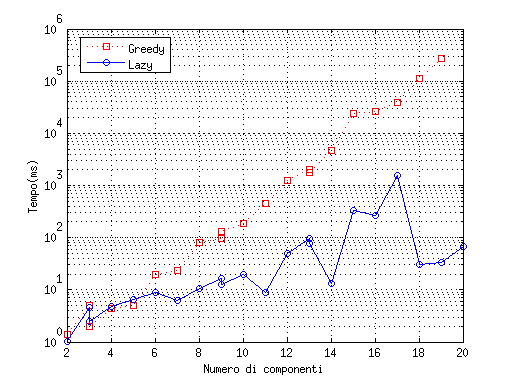
\includegraphics[scale=0.7]{./Img/sperimentazione/confronto_tempo.png}
\caption{Confronto dei tempi di esecuzione tra la diagnosi greedy e lazy}
\label{fig:confronto_tempo}
\end{figure}

\subsection{Memoria}
In figura \ref{fig:confronto_ram} viene analizzata, tramite un diagramma cartesiano, la differenza tra i due metodi diagnostici per quanto riguarda la memoria allocata. L'asse delle ascisse indica il numero di componenti dell'istanza, mentre l'asse verticale indica, in scala logaritmica, la memoria. Anche in questo caso, il metodo lazy non segue l'andamento esponenziale della diagnosi greedy. Ad esempio, per l'ultima istanza confrontabile di 19 componenti, il metodo greedy occupa 3.3GB, mentre l'algoritmo lazy utilizza solamente 10.5MB. L'istanza successiva di 20 componenti satura la memoria nel caso greedy, mentre con il metodo lazy sono sufficienti meno di 10MB.

\begin{figure}[htbp]
\centering
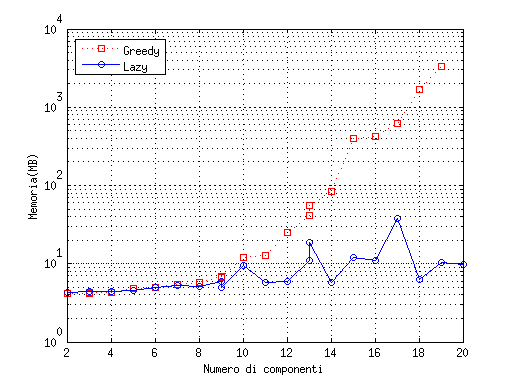
\includegraphics[scale=0.7]{./Img/sperimentazione/confronto_ram.png}
\caption{Confronto della memoria allocata tra la diagnosi greedy e lazy}
\label{fig:confronto_ram}
\end{figure}

\section{Approfondimento del metodo lazy}
Una volta verificata l'impraticabilità della diagnosi greedy, è stata effettuata una serie di esperimenti volti a catturare la complessità dell'algoritmo lazy.
In tabella \ref{tab:lazy_test} sono riportati i tempi di esecuzione e la memoria allocata per istanze di SAC con un numero di componenti che varia da 9 a 638, e un numero di nodi del sistema compreso tra 4 e 255.
Si noti che quasi tutte le istanze utilizzate, eccetto le prime due di 9 e 18 componenti, non siano calcolabili attraverso il metodo greedy. Uno stato del behavior del SAC nella sua interezza infatti, potrebbe nel caso peggiore aver un numero di stati, considerando ad esempio l'ultima istanza, esponenziale rispetto ai 638 componenti. 
Per mezzo del metodo lazy, i risultati per l'istanza più grande utilizzata (638 componenti e 255 nodi) sono di 3.209s di calcolo e 68.87MB di memoria allocata.
Sebbene sia chiaro che la complessità dell'algoritmo di ricostruzione del behavior sia esponenziale all'interno del singolo nodo che compone il SAC, è risultato che l'aggiunta di nodi al sistema non comporta una crescita esponenziale di risorse. Al contrario, i tempi di esecuzione si mantengono lineari nel numero di nodi del sistema e, per nodi di dimensione costante, l'andamento è lineare anche rispetto al numero di componenti. Questo andamento è facilmente osservabile nella figura \ref{fig:lazy_test_a} e \ref{fig:lazy_test_b}, rispettivamente per quanto riguarda il tempo di esecuzione e la RAM utilizzata.

\begin{table}[htbp] 
\begin{tabularx}{\textwidth}{X X X X}
\hline
Componenti & Nodi & Tempo(ms) & Memoria(MB)\\
\hline
9   &   4 & 16.68 &  5.88\\
18  &   7 & 37.27 &  6.28\\
27  &  10 & 59.38 &  6.86\\
38  &  15 & 87.79 &  7.82\\    
56  &  21 &   142 &  9.08\\
78  &  31 &   302 & 11.84\\
158 &  63 &   751 & 19.87\\
318 & 127 &  1615 & 36.18\\
638 & 255 &  3209 & 68.87\\
\hline
\end{tabularx}
\caption{Risultati dei test riguardanti il metodo lazy}
\label{tab:lazy_test}
\end{table}


\begin{figure}[htbp]
\centering
\subfigure[Tempo di esecuzione\label{fig:lazy_test_a}]
{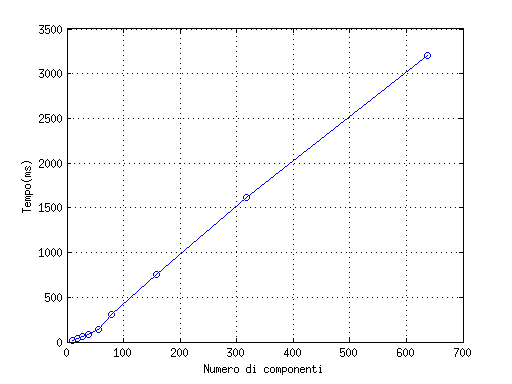
\includegraphics[scale=0.7]{./Img/sperimentazione/tempo_lazy.png}}
\hspace{5mm}
\subfigure[Memoria allocata\label{fig:lazy_test_b}]
{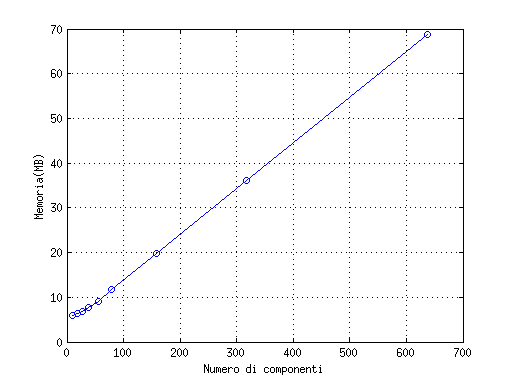
\includegraphics[scale=0.7]{./Img/sperimentazione/ram_lazy.png}}
\caption{Risultati dei test riguardanti il metodo lazy}
\label{fig:lazy_test}
\end{figure}
\chapter{Sviluppi futuri}
\chapter{Conclusioni}
Il lavoro svolto ha raggiunto gli obiettivi che erano stati prefissati.
Da un lato è stato definito un nuovo insieme di sistemi a eventi discreti, chiamati sistemi attivi complessi (SAC) e ne è stata fornita una specifica formale. I SAC sono stati concepiti come estensione dei sistemi attivi tradizionali, in quanto formati da una rete di questi ultimi, secondo una topologia gerarchica. Questo modello è stato suggerito dal comportamento di molti sistemi reali che possono essere descritti a diversi livelli di astrazione. 
D'altro canto è stato sviluppato un software in grado di calcolare le diagnosi di questi nuovi sistemi, secondo due metodi risolutivi. Il metodo greedy è stato ottenuto come naturale ampliamento dell'algoritmo diagnostico dei sistemi attivi tradizionali, mentre il metodo lazy è stato concepito al fine di migliorarne l'efficienza. Il confronto sperimentale tra le due tecniche, infatti, ha mostrato come a fronte di una crescita delle dimensioni del sistema, l'algoritmo greedy fosse inefficiente, consumando una quantità di memoria e un tempo di esecuzione esponenziali nel numero di componenti totali. L'algoritmo lazy, invece, non possiede un comportamento siffatto, ma trae vantaggio dalla topologia del sistema e produce la diagnosi in un unico passo bottom-up lungo la gerarchia del sistema. La complessità di questo algoritmo si stabilizza alla linearità per nodi di dimensione costante, potendo risolvere problemi che attraverso il metodo greedy non sarebbero affrontabili nella pratica.
A fronte di questi risultati positivi, il lavoro svolto può essere esteso in molteplici direzioni.

\newpage
\section{Sviluppi futuri}

\subsection{Parallelizzazione della diagnosi lazy}
Il metodo di diagnosi lazy ricostruisce in successione i comportamenti dei singoli nodi che compongono il sistema, seguendo un ordinamento topologico dell'albero che caratterizza l'interazione dei nodi. Un ordinamento topologico totale, tuttavia, non è strettamente necessario, in quanto è sufficiente fornire un ordinamento parziale. Il calcolo dei behavior non vincolati è eseguito uno indipendentemente dall'altro; questo suggerisce in modo naturale una parallelizzazione in fase diagnostica. Una volta ricostruiti i comportamenti dei nodi foglia, allo stesso modo il livello superiore della gerarchia è composto da nodi che, sebbene siano vincolati dal comportamento dei nodi sottostanti, non sono vincolati tra loro. Anche la ricostruzione del loro comportamento, quindi, può avvenire in parallelo. Procedendo in questo modo, è possibile effettuare una diagnosi in parallelo sui diversi nodi appartenenti allo stesso livello dell'albero. Questo metodo se implementato, causerebbe un ulteriore miglioramento nelle prestazioni del calcolo, rendendo l'algoritmo linearmente dipendente dal numero di livelli nella topologia del sistema, piuttosto che dal numero di nodi totale. 

\subsection{Aumento del preprocessing}
La fase di preprocessing permette di effettuare dei calcoli in fase di modellazione, evitando di spendere risorse nella successiva fase di diagnosi. L'aumento del calcolo in fase precedente potrebbe consistere nella generazione delle interfacce, la quale può richiedere delle risorse computazionali in alcuni casi costose, trattandosi di un algoritmo analogo alla subset construction. Attualmente le interfacce sono generate a partire dai behavior dei nodi, ma nulla vieta che tali interfacce possano essere generate partendo dai behavior space, che descrivono il comportamento prescindendo dall'osservazione, nota soltanto nella successiva diagnosi. Sebbene la generazione del behavior space è stata scartata nel metodo greedy poiché non praticabile nemmeno offline, la costruzione del behavior space del singolo nodo non dovrebbe essere altrettanto estenuante, assumendo una dimensione del singolo nodo limitata. In fase diagnostica le transizioni di interfaccia attuabili dovranno però essere selezionate in base all'osservazione data: parte delle interfacce costituirà una evoluzione inconsistente con l'osservazione temporale ed andrà scartata. Si noti che in letteratura sono presenti metodi diagnostici che calcolano un automa, detto diagnosticatore, derivato dal behavior space dell'intero sistema. Sebbene questo renda la successiva diagnosi lineare, la generazione di tale automa offline non è praticabile per problemi di dimensione reale.


\subsection{Variazioni nella topologia del sistema}
Nell'ambito di questo lavoro di tesi è stato analizzato il caso di sistemi attivi connessi tra loro in maniera gerarchica, formando un albero. Questa topologia particolare, tuttavia, può essere facilmente estesa al caso più generale di grafo aciclico. Anche in questo contesto è possibile ricostruire il comportamento dei nodi non vincolati, proseguendo in modo analogo a quanto descritto nella trattazione. Un'attenzione particolare deve essere prestata, tuttavia, nel caso in cui un nodo abbia più di un genitore, cioè influenzi più di un altro nodo del sistema. In questo caso la ricostruzione dei behavior dei nodi genitori deve essere effettuata in maniera sincronizzata, nel senso che un cambiamento di stato dell'interfaccia relativa al nodo figlio deve valere contemporaneamente  per tutti i nodi padre, altrimenti la diagnosi potrebbe avere delle soluzioni aggiuntive non sound. La ricostruzione prosegue allo stesso modo del caso di topologia ad albero: se vi sono più nodi radice, il behavior di ognuno di questi deve essere decorato, e le rispettive diagnosi combinate tra loro.\\
Un problema più complicato si verifica quando il sistema costituisce un generico grafo ciclico. In questo caso non è possibile effettuare semplicemente un processo bottom-up: si sceglie un nodo di partenza, si ricostruisce il comportamento relativo e la corrispondente diagnosi; successivamente, in caso esso sia influenzato da un altro nodo, il comportamento e l'interfaccia verranno potati opportunamente, in modo da essere consistenti con i pattern event ricevuti. Il processo quindi si sviluppa percorrendo i link che collegano i nodi un numero finito di volte, fino a quando il pruning non raggiunge una situazione di stabilità. 

\subsection{Osservazioni incerte}
In questo lavoro, le osservazioni dei nodi sono assunte essere sequenze lineari di label osservabili. In sistemi reali, tuttavia, un'osservazione potrebbe consistere in un ordinamento parziale delle label ricevute, anziché un ordinamento totale. In questo caso l'osservazione sarebbe percepita come un grafo orientato aciclico, invece di una semplice sequenza. Altri tipi di incertezze potrebbero riguardare il contenuto dell'osservazione: una label incerta potrebbe essere presente o meno nell'osservazione. Una volta delineato il grafo aciclico relativo all'osservazione, la consumazione di essa può essere monitorata generando un corrispondente automa, chiamato \emph{index space}, le cui transizioni sono percorse in corrispondondenza delle label osservate.


\subsection{Monitoring}
Nell'ambito di questo lavoro il focus è sulla cosiddetta diagnosi a posteriori, la quale avviene dopo un'osservazione completa del sistema, a seguito della quale viene calcolato l'insieme di diagnosi candidate. In un sistema reale, come ad esempio una centrale nucleare o una rete elettrica nazionale, il sistema difficilmente può essere pensato in uno stato quiescente a seguito del quale operare la diagnosi. L'osservazione in questi casi verrà ricevuta passo a passo e il compito della diagnosi, detta in questo ambito monitoring, consiste nel dare a seguito di una singola label di osservazione le diagnosi candidate in tempo reale, durante l'evoluzione del sistema. Estendendo il lavoro in questa direzione si potrebbe dare un metodo utile in applicazioni reali di questo tipo.

\appendix
\chapter{Automi a stati finiti}
Nell'ambito della diagnosi di sistemi a eventi discreti in generale e dei sistemi attivi (complessi) in particolare, il comportamento del sistema è descritto da successioni di eventi. A questo livello di astrazione, le sequenze di transizioni che si verificano possono essere rappresentate da un automa a stati finiti. Anche il comportamento dei singoli componenti del sistema, come si vedrà in seguito, può essere visto attraverso un automa. La semplicità e l'intuitività degli automi rende agevole il loro utilizzo in problemi di questo tipo, nonché nella più ampia branca dell'intelligenza artificiale.
Gli automi a stati finiti sono utili per una grande varietà di scopi, ad esempio per scansionare dei testi alla ricerca di parole o pattern, oppure nei compilatori per compiere la fase di analisi lessicale.
Gli automi sono anche detti riconoscitori, poiché ricevendo una stringa in ingresso, possono confermare o meno l'appartenenza di tale stringa al linguaggio definito dall'automa.
Esistono due principali tipi di automi a stati finiti:
\begin{itemize}
\item automi a stati finiti deterministici (DFA);
\item automi a stati finiti non deterministici (NFA).
\end{itemize}
In questo capitolo vengono presentati definizioni ed esempi riguardanti entrambe le classi di automi. In particolare, è descritto come convertire espressioni regolari in NFA e come convertire NFA in DFA.
Da ultimo viene fornito il concetto di automa minimo, cioè un automa caratterizzato dal minor numero di stati possibile, utile per una implementazione efficiente in termini di risorse computazionali.

\newpage
\section{DFA}
Un automa a stati finiti deterministico (DFA: deterministic finite automaton) è una quintupla:
\begin{center}
	$D = (\Sigma,S,t,s_0,F)$
\end{center}
dove:
\begin{itemize}
\item $\Sigma$ è un alfabeto, ovvero l'insieme dei simboli di input;
\item $S$ è un insieme finito di stati;
\item $t$ è la funzione di transizione (deterministica) $t: S \times \Sigma \rightarrow S$ che associa, ad uno stato e un simbolo di input, un nuovo stato;
\item $s_0$ è lo stato iniziale;
\item $F \subseteq S$ è un insieme di stati finali.
\end{itemize}
Un automa di questo tipo è detto deterministico poiché la sua funzione di transizione non permette l'esistenza, a partire da un medesimo stato, di due transizioni caratterizzate dallo stesso simbolo: l'automa, istantaneamente, si trova in un singolo stato.\\
Esistono due principali rappresentazioni per gli automi:
\begin{itemize}
\item tabella delle transizioni, rappresentazione tabellare della funzione di transizione dove nelle righe si trovano gli stati di partenza, mentre nelle colonne i simboli (o viceversa). L'elemento in una cella della tabella rappresenta lo stato destinazione della transizione, a partire dallo stato della riga corrispondente e in base al simbolo di input nella relativa colonna; particolari notazioni grafiche possono essere utilizzate per contraddistinguere lo stato iniziale e gli stati finali.
\item diagramma delle transizioni, un grafo nel quale:
	\begin{itemize}
	\item ogni stato è rappresentato da un vertice;
	\item ogni transizione è un arco orientato che connette due vertici e possiede una label indicante il simbolo della transizione;
	\item una freccia entrante in un vertice rappresenta lo stato iniziale;
	\item ogni vertice associato ad uno stato finale è descritto da un doppio contorno, mentre gli stati non finali hanno come vertice un contorno singolo.
	\end{itemize}
\end{itemize}

\begin{ex}
Si consideri un DFA con $\Sigma = \{ a,b\}$, $S = \{ s_0,s_1,s_2\}$, stato iniziale $s_0$, insieme di stati finali $F = \{s_2\}$ e funzione di transizione $t$ che si evince dalle rappresentazioni in tabella \ref{tab:dfa} e figura \ref{fig:dfa}.

\begin{table}[htbp]
\begin{center}
\begin{tabular}{r | c  c}
& a & b \\ \hline
$\rightarrow s_0$ & $s_1$ & $s_0$ \\
$s_1$ & $s_1$ & $s_2$ \\
$*s_2$ & $s_2$ & $s_2$ 
\end{tabular}
\caption{Rappresentazione tramite tabella di un DFA}
\label{tab:dfa}
\end{center}
\end{table}


\begin{figure}[htbp]
\centering
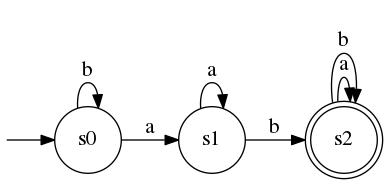
\includegraphics[scale=0.4]{./Img/automi/ex1.png}
\caption{Rappresentazione grafica di un DFA}
\label{fig:dfa}
\end{figure}

\end{ex}

\subsection{Linguaggio di un DFA}
Il linguaggio di un DFA è l'insieme di tutte le stringhe che il DFA accetta. 
Sia $a_1, a_2, \dots, a_n$ una sequenza di simboli. A partire dallo stato iniziale $s_0$, mediante la funzione di transizione $t$ si ha $s_1 = t(s_0, a_1)$ come stato raggiunto a fronte dell'ingresso $a_1$. Procedendo allo stesso modo per altri simboli, $s_i = t(s_{i-1}, a_i)$, si viene a creare una sequenza di stati raggiunti  $s_1, s_2, \dots, s_n$. La sequenza è accettata se e solo se si raggiunge uno stato finale $s_n \in F$.
\'E possibile introdurre il concetto di \emph{funzione di transizione estesa} che restituisce lo stato raggiunto quando a partire da uno stato si ha una sequenza di simboli d'ingresso, invece che un simbolo soltanto. La funzione di transizione estesa $\hat t: S \times \Sigma^* \mapsto S$ è definita come:
$$
\hat t(s, \underline \omega) = \begin{cases}
s & \underline \omega = \epsilon,\\
t(\hat t(q, \underline x), a) & \underline \omega = \underline x\,a
\end{cases}
$$

Dunque una stringa $\underline \omega = a_1\, a_2\,\dots\,a_n$ appartiene al linguaggio definito dall'automa se e solo se $\hat t(s_0, \underline \omega) \in F$.
Di conseguenza si definisce linguaggio del DFA $D = (S,\Sigma, t, s_0, F)$:
$$
L(D) = \{\,\underline \omega\,\,|\,\,\hat t(s_0, \underline \omega) \in F\,\}.
$$

\newpage
\section{NFA}
Un automa a stati finiti non deterministico (NFA: nondeterministic finite automaton) è una quintupla:
\begin{center}
	$N = (\Sigma,S,t,s_0,F)$
\end{center}
dove:
\begin{itemize}
\item $\Sigma$ è un alfabeto, ovvero l'insieme dei simboli di input;
\item $S$ è un insieme finito di stati;
\item $t$ è la funzione di transizione (non deterministica) $t: S \times (\Sigma \cup \{\epsilon\}) \rightarrow 2^S$ che associa, ad uno stato e un simbolo di input (oppure al simbolo vuoto $\epsilon$), un insieme di stati;
\item $s_0$ è lo stato iniziale;
\item $F \subseteq S$ è un insieme di stati finali.
\end{itemize}
La differenza tra gli automi deterministici e quelli non deterministici riguarda la funzione di transizione, che in quest'ultima classe di automi presenta due forme di non determinismo: da un lato, la presenza di $\epsilon$-transizioni può causare il cambiamento di stato dell'automa senza che venga consumato alcun simbolo in input; d'altro canto, la possibile presenza di transizioni uscenti dal medesimo stato con la stessa label fornisce una scelta non deterministica nella simulazione dell'automa.
Il teorema che è analizzato nella sezione successiva mostra che è sempre possibile, partendo da un NFA, ricostruire un corrispondente DFA equivalente.
L'utilizzo di automi non deterministici è dettato dalla maggior facilità di modellazione nell'ambito di alcuni algoritmi specifici, nonché da procedure note che permettono di costruire un automa non deterministico equivalente ad una espressione regolare data \footnote{Si noti che, come illustrato in \cite{book:compilers}, è altresì possibile partendo da un'espressione regolare costruire direttamente un DFA.}.\\
Le possibili rappresentazioni di NFA sono simili a quelle viste per i DFA, con piccole variazioni: nella rappresentazione tabellare ogni cella, invece che contenere un singolo stato, racchiude un insieme di stati, e come simboli si aggiunge una colonna che esplicita le transizioni scatenate dal simbolo vuoto; nella rappresentazione grafica, si ricorre a frecce con la label $\epsilon$ per indicare le $\epsilon$-transizioni.

\begin{ex}
Viene di seguito riportato un esempio di NFA.

\begin{table}[htbp]
\begin{center}
\begin{tabular}{r | c  c  c}
& a & b & $\epsilon$ \\ \hline
$\rightarrow s_0$ & $\emptyset$ & $\{s_4\}$ & $\{s_1,s_2,s_3\}$\\
$s_1$ & $\{s_4\}$ & $\emptyset$ & $\{s_3\}$\\
$s_2$ & $\emptyset$ & $\{s_3\}$ & $\emptyset$\\ 
$*s_3$ & $\emptyset$ & $\{s_4\}$ & $\emptyset$\\ 
$*s_4$ & $\{s_3\}$ & $\emptyset$ & $\emptyset$\\
\end{tabular}
\caption{Rappresentazione tramite tabella di un NFA}
\label{tab:nfa}
\end{center}
\end{table}

\begin{figure}[htbp]
\centering
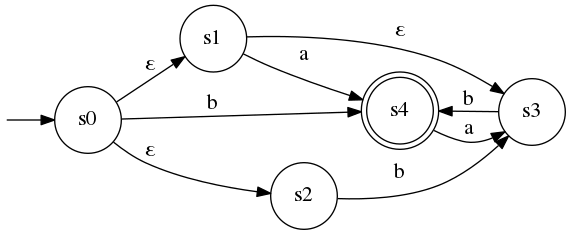
\includegraphics[scale=0.4]{./Img/automi/nfa.png}
\caption{Rappresentazione grafica di un NFA}
\label{fig:nfa}
\end{figure}

\end{ex}

\subsection{\texorpdfstring{$\epsilon$}-closure}
La $\epsilon$-closure di uno stato $s$ è l'insieme degli stati raggiunti a partire da $s$ tramite transizioni di stato senza simboli di input, ovvero mediante $\epsilon$-transizioni.
Formalmente $\epsilon\textit{-closure} : S \mapsto 2^S$ tale che:
$$
\epsilon\textit{-closure}(s) = \begin{cases}
\{s\} & t(s, \varepsilon) = \emptyset \\
\{s\} \cup \displaystyle \bigcup_{s_i \in A} \epsilon\textit{-closure}(s_i) & A = t(s, \varepsilon) \ne \emptyset
\end{cases}
$$
\'E inoltre possibile introdurre la nozione di $\epsilon$-closure per insiemi di stati, $\epsilon\textit{-closure}^*: 2^S \mapsto 2^S$:
$$
\epsilon\textit{-closure}^*(\mathbb{T} \subseteq S) = \displaystyle\bigcup_{s_i \in \mathbb{T}} \epsilon\textit{-closure}(s_i)
$$

\subsection{Linguaggio di un NFA}
Attraverso il concetto di $\epsilon$-closure è possibile definire in modo conciso la \emph{funzione di transizione estesa} per stringhe non contenenti il simbolo $\varepsilon$. 
Si definisce $\hat t:  S \times \Sigma^* \mapsto 2^S$:
$$
\hat t(s, \underline \omega) = \begin{cases}
\mathcal{E}\textit{-closure}(s) & \omega = \epsilon \\
\mathcal{E}\textit{-closure}^*(A) & \omega = \underline x \, a \,,\, A=\displaystyle\bigcup_{s_i \in B} t(s_i, a)\,,\,B=\hat t(s, \underline x)
\end{cases}
$$

Dunque una stringa $\underline \omega = a_1\, a_2\,\dots\,a_n$ appartiene al linguaggio definito dall'automa se e solo se $\hat t(s_0, \underline \omega) \in F$.

Di conseguenza si definisce linguaggio del NFA $N = (S,\Sigma, t, s_0, F)$:
$$
L(N_\varepsilon) = \{\,\underline \omega\,\,|\,\,\hat t(s_0, \underline \omega) \cap F \ne \emptyset\,\}.
$$


\newpage
\section{Subset construction}
A causa del loro non determinismo, spesso i NFA necessitano di essere convertiti in DFA per essere utilizzati e simulati in modo più intuitivo. La tecnica nota in letteratura per ottenere questa conversione è chiamata \emph{subset construction}.
L'idea generale di questo algoritmo è che ad ogni stato del risultante DFA corrisponde un insieme di stati del NFA di partenza.
Il primo problema che bisogna affrontare è quello di gestire le $\epsilon$-transizioni. Queste particolari transizioni indicano in quali stati l'automa può trovarsi contemporaneamente. L'operazione di $\epsilon$-closure permette di trovare, a partire da un particolare stato, tutti gli stati raggiungibili senza la consumazione di simboli in ingresso. Il primo passo della subset construction, quindi, consiste nell'assegnare allo stato iniziale del DFA risultante la $\epsilon$-closure dello stato iniziale del NFA in esame. L'algoritmo prosegue calcolando, per ogni possibile input ricevuto a partire da ogni stato del NFA contenuto nello  stato attuale del DFA, l'insieme degli stati raggiungibili, su cui viene effettuata la $\epsilon$-closure. Il procedimento procede in questo modo sino a che tutti i nuovi stati generati nel DFA non sono stati processati. Lo pseudocodice è fornito nell'algoritmo \ref{alg:subset}.
\'E possibile, teoricamente, che il numero di stati del DFA sia esponenziale nel numero di stati del NFA: tale numero è limitato superiormente dalla cardinalità dell'insieme potenza degli stati dell'automa non deterministico, cioè dal numero di tutti i possibili sottoinsiemi degli stati.
Fortunatamente questo caso pessimo raramente si presenta e per linguaggi reali spesso il numero di stati dei due automi è simile e il comportamento esponenziale non sussiste.

\begin{algorithm}
\textbf{SubsetConstruction($N$)}
\begin{algorithmic}
\STATE Sia $s_0$ lo stato iniziale del NFA, $Dstates$ gli stati del DFA risultante, $t$ la funzione di transizione del DFA
\WHILE{$\exists s \in Dstates$ non marcato}
	\STATE marcare $s$
	\FORALL{simbolo di input $a$}
		\STATE $U = \epsilon-closure(move(T,a))$
		\IF{$U \notin Dstates$}
			\STATE aggiungi $U$ come stato non marcato in $Dstates$
		\ENDIF
		\STATE $t(T,a) = U$
	\ENDFOR
\ENDWHILE
\end{algorithmic}
\caption{Algoritmo subset construction}
\label{alg:subset}
\end{algorithm}

\newpage
\section{Linguaggi}
Un automa a stati finiti possiede delle transizioni i cui simboli costituiscono l'alfabeto di un linguaggio e una stringa ottenuta percorrendo un cammino dallo stato iniziale ad uno stato finale si dice che appartiene al linguaggio. Una stringa caratterizzata da nessun simbolo dell'alfabeto è detta stringa vuota e si denota con $\epsilon$.
Data una stringa $s$, la sua lunghezza $|s|$ è il numero di simboli contenuti in essa, tenendo conto di eventuali occorrenze multiple del medesimo simbolo. Per convenzione, la lunghezza della stringa vuota è zero.
\begin{defn}
Un linguaggio definito su un insieme alfabeto $\Sigma$ è un insieme di stringhe di lunghezza finita formate da simboli appartenenti a $\Sigma$.
\end{defn}
L'operazione fondamentale per la costruzione di linguaggi è quella della concatenazione. Se $x$ e $y$ sono stringhe, la loro concatenazione è la stringa $xy$. La stringa vuota è l'elemento identità di tale operazione, poiché per ogni stringa $s$, $s\epsilon = \epsilon s = s$.\\
Un'altra operazione che caratterizza i linguaggi è la chiusura di Kleene, denotata $L^*$, che è l'insieme di tutte le stringhe finite che si ottengono concatenando elementi dell'alfabeto, compresa la stringa vuota.\\
Sui linguaggi è altresì possibile applicare tutte le operazioni insiemistiche quali l'unione, l'intersezione, la differenza e il complemento.
Un linguaggio può essere visto come un modo formale di descrivere il comportamento di un sistema, specificando tutte le possibili sequenze di eventi che esso è in grado di generare. 
Un automa è un formalismo in grado di rappresentare un linguaggio.
In particolare, nel seguito della trattazione, ci si focalizzerà sui cosiddetti linguaggi regolari, ovvero su quei linguaggi che possono essere rappresentati tramite automi con un numero finito di stati.

\section{Espressioni regolari}
Le espressioni regolari costituiscono quell'insieme di linguaggi che possono essere rappresentati da automi a stati finiti (grammatica di tipo 3 della gerarchia di Chomsky). Le espressioni regolari descrivono tutti i linguaggi costruiti applicando ai simboli appartenenti ad un alfabeto $\Sigma$ gli operatori di unione, concatenazione e chiusura. Le espressioni regolari sono generate ricorsivamente dalle sottoespressioni che le formano, secondo le seguenti regole.
\begin{enumerate}
\item $\epsilon$ è una espressione regolare che denota il linguaggio $L(\epsilon) = \{\epsilon\}$, 					contenente la sola stringa vuota;
\item se $a$  è un simbolo in $\Sigma$, allora $a$ è un'espressione regolare che denota il linguaggio $L(a) = 	\{a\}$, contenente la sola stringa di lunghezza unitaria $a$.
\item se $x$ e $y$ sono espressioni regolari che denotano rispettivamente i linguaggi $L(x)$ e $L(y)$, allora:
	\begin{itemize}
	\item $(x)$ è l'espressione regolare che denota il linguaggio $L(x)$;
	\item $(x) | (y)$ è l'espressione regolare che denota il linguaggio $L(x) \cup L(y)$ (unione);
	\item $(x)(y)$ è l'espressione regolare che denota il linguaggio $L(x)L(y) = \{xy | x \in L(x), y \in L(y)\}$ (concatenazione);
	\item $(x)^*$ è l'espressione regolare che denota il linguaggio $(L(x))^*$: ripetizione zero o più volte di stringhe in $L(x)$ (chiusura di Kleene).
	\end{itemize}
\end{enumerate}
Altri operatori possono essere definiti opportunamente in base al dominio applicativo, generando espressioni regolari estese.

\subsection{Costruzione di Thompson}
La costruzione di \emph{McNaughton- Yamada- Thompson}(o semplicemente costruzione di Thompson) è in grado di convertire una espressione regolare in un NFA caratterizzato dal medesimo linguaggio. L'algoritmo opera scomponendo l'espressione regolare in un albero sintattico e costruendo un NFA per ogni sottoespressione, in maniera bottom-up, utilizzando le $\epsilon$-transizioni come "collante" per unire i sottoautomi. L'automa risultante permette di riconoscere se una stringa appartiene o meno al linguaggio relativo all'espressione regolare di partenza.\\
La regola base del metodo, rappresentata in figura \ref{fig:re_atom}, genera un NFA da una sottoespressione atomica, composta da un solo simbolo $a$ o dal simbolo nullo $\epsilon$. L'automa generato è composto da due stati, uno iniziale e l'altro finale, e una transizione in corrispondenza del simbolo atomico dallo stato iniziale allo stato finale.
Le regole induttive permettono di ricavare ricorsivamente l'intero automa.
Si supponga che $N(s)$ e $N(t)$ siano gli NFA ricavati dalle espressioni regolari $s$ e $t$ rispettivamente.
\begin{enumerate}
\item Si supponga $r = s|t$. L'automa $N(r)$ equivalente all'espressione regolare $r$ è costruito in figura \ref{fig:re_union}. Sono creati due nuovi stati, uno iniziale e uno finale. Due $\epsilon$-transizioni uniscono lo stato iniziale del nuovo automa agli stati iniziali di $N(r)$ e $N(s)$. Si noti che gli stati finali di $N(r)$ e $N(s)$ non sono finali nel nuovo automa, e una $\epsilon$-transizione collega ciascuno al nuovo stato finale. Il linguaggio dell'automa generato è l'unione dei linguaggi dei due automi di partenza.
\item Si supponga $r = st$. L'automa $N(r)$ equivalente all'espressione regolare $r$ è costruito in figura \ref{fig:re_concat}. Lo stato iniziale di $N(s)$ diviene in nuovo stato iniziale di $N(r)$, mentre lo stato finale di $N(t)$ costituisce il nuovo stato finale dell'automa risultante $N(r)$ . Il linguaggio dell'automa generato è la concatenazione dei linguaggi dei due automi di partenza.
\item Si supponga $r = s^*$. L'automa $N(r)$ equivalente all'espressione regolare $r$ è costruito in figura \ref{fig:re_closure}. Sono creati due nuovi stati, uno iniziale e uno finale. A partire dallo stato iniziale, vengono poste due $\epsilon$-transizioni: una verso lo stato iniziale di $N(s)$, l'altra verso il nuovo stato finale. Inoltre è aggiunta una $\epsilon$-transizione dallo stato finale per $N(s)$ al suo stato iniziale per $N(s)$. Il linguaggio dell'automa generato dalla chiusura di Kleene dei linguaggi dei due automi di partenza.
\item Si supponga $r = (s)$. Allora il linguaggio di $r$ coincide con quello di $s$, e come automa $N(r)$ può essere utilizzato l'automa di partenza $N(s)$.
\end{enumerate} 


\begin{figure}[htbp]
\centering
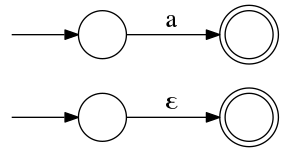
\includegraphics[scale=0.4]{./Img/automi/re_atom.png}
\caption{NFA per espressioni regolari atomiche}
\label{fig:re_atom}
\end{figure}


\begin{figure}[htbp]
\centering
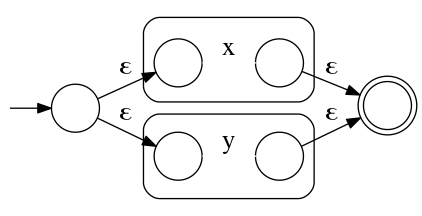
\includegraphics[scale=0.4]{./Img/automi/re_union.png}
\caption{NFA per l'unione di due espressioni regolari}
\label{fig:re_union}
\end{figure}

\begin{figure}[htbp]
\centering
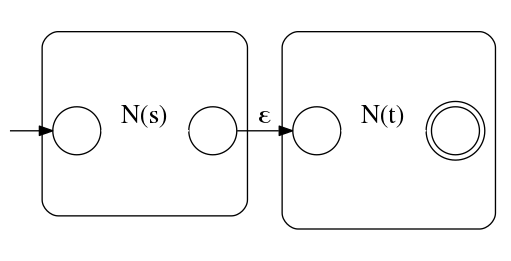
\includegraphics[scale=0.4]{./Img/automi/re_concat.png}
\caption{NFA per la concatenazione di due espressioni regolari}
\label{fig:re_concat}
\end{figure}

\begin{figure}[htbp]
\centering
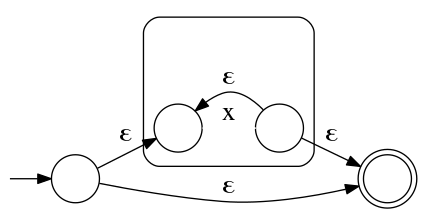
\includegraphics[scale=0.4]{./Img/automi/re_closure.png}
\caption{NFA per la chiusura di un'espressione regolare}
\label{fig:re_closure}
\end{figure}


\newpage
\section{Minimizzazione degli stati}
Dato un linguaggio, possono esistere più automi deterministici che lo riconoscono. Si cerca sempre di scegliere l'automa che presenta il minor numero di stati, dato che l'implementazione di quest'ultimo consente di risparmiare memoria e tempo nella simulazione. 
Esiste sempre un unico DFA minimo per ogni linguaggio regolare, a meno di una ridenominazione del nome degli stati. Questo particolare automa può essere costruito raggruppando insieme quegli stati che sono tra loro equivalenti. Per capire come verificare tale equivalenza, si ricorre al concetto di distinguibilità.
\begin{defn}
La stringa $x$ distingue lo stato $s$ dallo stato $t$ se esattamente uno degli stati raggiunti partendo da $s$ e da $t$ seguendo il cammino con label $x$ è uno stato finale. Quindi, lo stato $s$ è distinguibile dallo stato $t$ se esiste una stringa che li distingue.
In particolare, la stringa vuota distingue ogni stato finale da qualsiasi stato non finale.
\end{defn}

L'algoritmo di minimizzazione degli stati funziona partizionando gli stati dell'automa in gruppi di stati indistinguibili. 
In ogni istante, l'algoritmo mantiene partizioni di stati che non sono ancora stati distinti.
Inizialmente gli stati sono divisi in due macro-partizioni, una contenente gli stati non finali, l'altra contente quelli finali. La divisione iniziale viene raffinata individuando un simbolo di input che distingue tra loro alcuni degli stati appartenenti ad un gruppo, generando in questo modo una ulteriore suddivisione interna. La procedura viene applicata fino a quando nessun gruppo, per ogni simbolo di input, può essere scisso nuovamente.
Infine ogni gruppo di stati, scegliendo per ogni insieme uno stato come rappresentante, viene fuso in un singolo stato che appartiene all'automa minimo risultante. 

\listoffigures

\nocite{*}
\bibliographystyle{unsrt}
\bibliography{bibliografia}
\addcontentsline{toc}{chapter}{\bibname}

\end{document}